% ============================================================
%  TG – Instituto Tecnológico de Aeronáutica
%  Engenharia Mecânica
%  Previsão de Geração Fotovoltaica com Aprendizado de Máquina
% ============================================================
\documentclass[
  12pt,
  openright,
  twoside,
  a4paper,
  brazil,
  % english,   % descomente se redigir em inglês
]{abntex2}

% ------------------------------------------------------------
% Pacotes essenciais
% ------------------------------------------------------------
\usepackage[T1]{fontenc}
\usepackage[utf8]{inputenc}
\usepackage{mathptmx}          % Times New Roman (texto + math)
\usepackage{microtype}
\usepackage{indentfirst}
\usepackage{color}
\usepackage{graphicx}
\usepackage{booktabs}
\usepackage{tabularx}
\usepackage{multirow}
\usepackage{amsmath, amssymb}
\usepackage{siunitx}           % unidades SI: \SI{100}{\watt}
\usepackage{eurosym}           % símbolo \euro
\DeclareSIUnit\kWh{kWh}
\DeclareSIUnit\kWp{kWp}
\DeclareSIUnit\peak{p}         % watt-pico: \watt\peak = Wp
\sisetup{per-mode=repeated-symbol} % permite \per múltiplo: kWh/kWp/dia
\usepackage{hyperref}
\usepackage[brazilian,hyperpageref]{backref}
\usepackage[alf,abnt-emphasize=bf]{abntex2cite}  % citações ABNT autor-data

% ------------------------------------------------------------
% Configuração de margens (ABNT: sup 3cm, inf 2cm, esq 3cm, dir 2cm)
% ------------------------------------------------------------
\usepackage[
  top=3cm,
  bottom=2cm,
  left=3cm,
  right=2cm
]{geometry}

% ------------------------------------------------------------
% Espaçamento entre linhas (1,5 – padrão ABNT)
% ------------------------------------------------------------
\OnehalfSpacing

% ------------------------------------------------------------
% Configuração do hyperref
% ------------------------------------------------------------
\hypersetup{
  pdftitle={Previsão de Geração de Energia Elétrica de Usinas
            Fotovoltaicas Utilizando Aprendizado de Máquina},
  pdfauthor={REBOUÇAS, Pedro},
  pdfsubject={Trabalho de Graduação - ITA},
  pdfkeywords={energia fotovoltaica, aprendizado de máquina,
               previsão de geração, séries temporais},
  colorlinks=true,
  linkcolor=black,
  citecolor=black,
  urlcolor=black
}

% ------------------------------------------------------------
% Informações do trabalho
% ------------------------------------------------------------
\titulo{Desenvolvimento de um Modelo de Previsão de Geração de
        Energia Elétrica de Usinas Fotovoltaicas Utilizando
        Aprendizado de Máquina}
\autor{Pedro Arthur Sales Rebouças}
\local{São José dos Campos}
\data{2026}
\instituicao{Instituto Tecnológico de Aeronáutica}
\tipotrabalho{Trabalho de Graduação}
\orientador{Prof.\ Dr.\ Rodrigo Arnaldo Scarpel (ITA)}
% \coorientador{Prof.\ Dr.\ Nome do Coorientador (INSTITUIÇÃO)}
\curso{Engenharia Mecânica}

\preambulo{Trabalho de Graduação apresentado ao Curso de
           Engenharia Mecânica do Instituto Tecnológico de
           Aeronáutica, como requisito parcial para obtenção do
           título de Engenheiro Mecânico.}

% ============================================================
\begin{document}
% ============================================================

% ------------------------------------------------------------
% Elementos pré-textuais
% ------------------------------------------------------------
\pretextual

\imprimircapa

\imprimirfolhaderosto*   % * = gera espaço para ficha catalográfica

% -- Ficha catalográfica (verso da folha de rosto) -----------
\begin{fichacatalografica}
  \vspace*{\fill}
  \begin{center}
    \fbox{
      \begin{minipage}[c][8cm]{13cm}
        \small
        \textbf{Dados Internacionais de Catalogação-na-Publicação (CIP)} \\
        \textbf{Divisão de Informação e Documentação} \\[6pt]
        REBOUÇAS, Pedro \\
        \hspace{0.5cm} \imprimirtitulo{} / \imprimirautor. \\
        \hspace{0.5cm} \imprimirlocal, \imprimirdata. \\
        \hspace{0.5cm} XX f. \\[6pt]
        \hspace{0.5cm} Trabalho de Graduação -- Curso de \imprimircurso{}
        -- \imprimirinstituicao, \imprimirdata. \\
        \hspace{0.5cm} Orientador: \imprimirorientador. \\[6pt]
        \hspace{0.5cm} 1. Energia fotovoltaica. 2. Aprendizado de máquina.
        3. Previsão de geração. \\
        \hspace{0.5cm} I. \imprimirinstituicao. II. Título.
      \end{minipage}
    }
  \end{center}
\end{fichacatalografica}

% -- Folha de aprovação --------------------------------------
\begin{folhadeaprovacao}
  \begin{center}
    {\large\bfseries\imprimirtitulo}\\[2cm]
    Esta publicação foi aceita como Relatório Final de Trabalho de Graduação\\[2cm]
    \makebox[10cm]{\hrulefill}\\
    \imprimirautor\\
    Autor\\[1.5cm]
    \makebox[10cm]{\hrulefill}\\
    \imprimirorientador\\
    Orientador\\[1.5cm]
    \imprimirlocal, \the\year
  \end{center}
\end{folhadeaprovacao}

% -- Dedicatória ---------------------------------------------
\begin{dedicatoria}
  \vspace*{\fill}
  \begin{flushright}
    \textit{Dedique este trabalho a quem desejar.}
  \end{flushright}
\end{dedicatoria}

% -- Agradecimentos ------------------------------------------
\begin{agradecimentos}
  Escreva aqui seus agradecimentos.
\end{agradecimentos}

% -- Epígrafe (opcional) -------------------------------------
\begin{epigrafe}
  \vspace*{\fill}
  \begin{flushright}
    \textit{``Frase inspiradora opcional.''}\\
    (Autor da frase)
  \end{flushright}
\end{epigrafe}

% -- Resumo --------------------------------------------------
\setlength{\absparsep}{18pt}
\begin{resumo}
  Escreva aqui o resumo em português (máximo 500 palavras, conforme ABNT NBR 6028:2021).
  O resumo deve apresentar de forma concisa os objetivos, metodologia, resultados e
  conclusões do trabalho.

  \noindent\textbf{Palavras-chave:} energia fotovoltaica; aprendizado de máquina;
  previsão de geração; séries temporais; usinas solares.
\end{resumo}

% -- Abstract ------------------------------------------------
\begin{resumo}[Abstract]
  \begin{otherlanguage*}{english}
    Write the abstract here (maximum 500 words).
    The abstract should present concisely the objectives, methodology, results and
    conclusions of the work.

    \noindent\textbf{Keywords:} photovoltaic energy; machine learning;
    generation forecasting; time series; solar power plants.
  \end{otherlanguage*}
\end{resumo}

% -- Listas --------------------------------------------------
\pdfbookmark[0]{\listfigurename}{lof}
\listoffigures*
\cleardoublepage

\pdfbookmark[0]{\listtablename}{lot}
\listoftables*
\cleardoublepage

% -- Lista de abreviaturas e siglas --------------------------
\begin{siglas}
  \item[ABNT]  Associação Brasileira de Normas Técnicas
  \item[ANN]   Artificial Neural Network (Rede Neural Artificial)
  \item[EPE]   Empresa de Pesquisa Energética
  \item[FV]    Fotovoltaico
  \item[GHI]   Global Horizontal Irradiance (Irradiância Horizontal Global)
  \item[ITA]   Instituto Tecnológico de Aeronáutica
  \item[LSTM]  Long Short-Term Memory
  \item[MAE]   Mean Absolute Error (Erro Absoluto Médio)
  \item[ML]    Machine Learning (Aprendizado de Máquina)
  \item[MAPE]  Mean Absolute Percentage Error
  \item[NWP]   Numerical Weather Prediction (Previsão Numérica do Tempo)
  \item[RMSE]  Root Mean Square Error (Raiz do Erro Quadrático Médio)
  \item[SFV]   Sistema Fotovoltaico
  \item[UFV]   Usina Fotovoltaica
  \item[XGBoost] Extreme Gradient Boosting
\end{siglas}

% -- Lista de símbolos (opcional) ----------------------------
\begin{simbolos}
  \item[$G$]       Irradiância solar [\si{\watt\per\square\meter}]
  \item[$P_{ac}$]  Potência CA gerada [\si{\watt}]
  \item[$P_{dc}$]  Potência CC gerada [\si{\watt}]
  \item[$T_{amb}$] Temperatura ambiente [\si{\celsius}]
  \item[$T_{mod}$] Temperatura do módulo fotovoltaico [\si{\celsius}]
  \item[$\eta$]    Eficiência do sistema fotovoltaico
  \item[$\hat{y}$] Valor previsto pelo modelo
  \item[$y$]       Valor real observado
\end{simbolos}

% -- Sumário -------------------------------------------------
\pdfbookmark[0]{\contentsname}{toc}
\tableofcontents*
\cleardoublepage

% ============================================================
% Elementos textuais
% ============================================================
\textual

% ============================================================
%  Capítulo 1 – Introdução
% ============================================================
\chapter{Introdução}
\label{cap:introducao}


\section{Cenário brasileiro de geração fotovoltaica}
\subsection{Dados atuais de geração}
\label{sec:cenario_brasileiro}

Segundo o Balanço Energético Nacional, divulgado em 2025 pela Empresa de
Pesquisa Energética (EPE), a energia solar fotovoltaica consolidou-se como a
fonte de maior crescimento da matriz brasileira nos últimos anos. Ao final de
2024, a capacidade instalada da fonte alcançou \SI{48,468}{\giga\watt},
representando uma expansão de \SI{28,1}{\percent} em relação ao ano anterior
\cite{EPE2025}. A geração de energia, consequentemente, também acompanhou esse ritmo, a produção solar fotovoltaica atingiu \SI{70,7}{\tera\watt\hour} em 2024, crescimento de
\SI{39,6}{\percent} sobre 2023 \cite{EPE2025}, conforme pode ser visto na Tabela \ref{tab:matriz_energetica}.

\begin{table}[htbp]
\centering
\caption{Geração de energia elétrica e capacidade instalada no Brasil, 2023--2024.}
\label{tab:matriz_energetica}
\begin{tabular}{lrrr}
\hline
\textbf{Fonte} & \textbf{2023} & \textbf{2024} & \textbf{$\Delta$\% 24/23} \\
\hline
\multicolumn{4}{l}{\textit{Geração (GWh)}} \\
\hline
Hidrelétrica          & 425.996 & 421.799 & $-$1,0\% \\
Gás Natural           &  38.589 &  47.792 & 23,9\%   \\
Eólica                &  95.801 & 107.654 & 12,4\%   \\
Biomassa              &  54.210 &  58.027 &  7,0\%   \\
Nuclear               &  14.504 &  15.767 &  8,7\%   \\
Carvão Vapor          &   8.770 &  10.247 & 16,8\%   \\
Derivados do Petróleo &   5.686 &   5.960 &  4,8\%   \\
\textbf{Solar Fotovoltaica} & \textbf{50.633} & \textbf{70.665} & \textbf{39,6\%} \\
Outras                &  13.932 &  13.425 & $-$3,6\% \\
\textbf{Geração Total}& \textbf{708.119} & \textbf{751.335} & \textbf{6,1\%} \\
\hline
\multicolumn{4}{l}{\textit{Capacidade Instalada (MW)}} \\
\hline
Hidrelétrica          & 109.922 & 109.922 &  0,0\%   \\
Térmica               &  47.515 &  46.439 & $-$2,3\% \\
Nuclear               &   1.990 &   1.990 &  0,0\%   \\
Eólica                &  28.682 &  29.550 &  3,0\%   \\
\textbf{Solar}        & \textbf{37.843} & \textbf{48.468} & \textbf{28,1\%} \\
\textbf{Capacidade Disponível} & \textbf{225.952} & \textbf{236.370} & \textbf{4,6\%} \\
\hline
\end{tabular}
\legend{Fonte: \citeonline{EPE2025}.}
\end{table}

Com efeito, ao caracterizar a inserção da fonte na matriz energética, é necessário distinguir
dois indicadores frequentemente confundidos. Em relação à matriz elétrica
nacional, na qual é contabilizada exclusivamente a geração de energia elétrica, a
solar respondeu por \SI{9,3}{\percent} do total em 2024 \cite{EPE2025}. Já em
relação à Oferta Interna de Energia (OIE), indicador mais amplo que abrange todas
as formas de energia consumidas no país, incluindo combustíveis para transporte e
processos industriais, a participação da fonte foi de \SI{2,2}{\percent}
\cite{EPE2025}. A diferença entre os dois percentuais é esperada e decorre da distinta abrangência de cada indicador e ao explicitá-la evita-se interpretações equivocadas sobre o real peso da fonte no sistema energético como um todo.

\begin{figure}[!h]
    \centering
    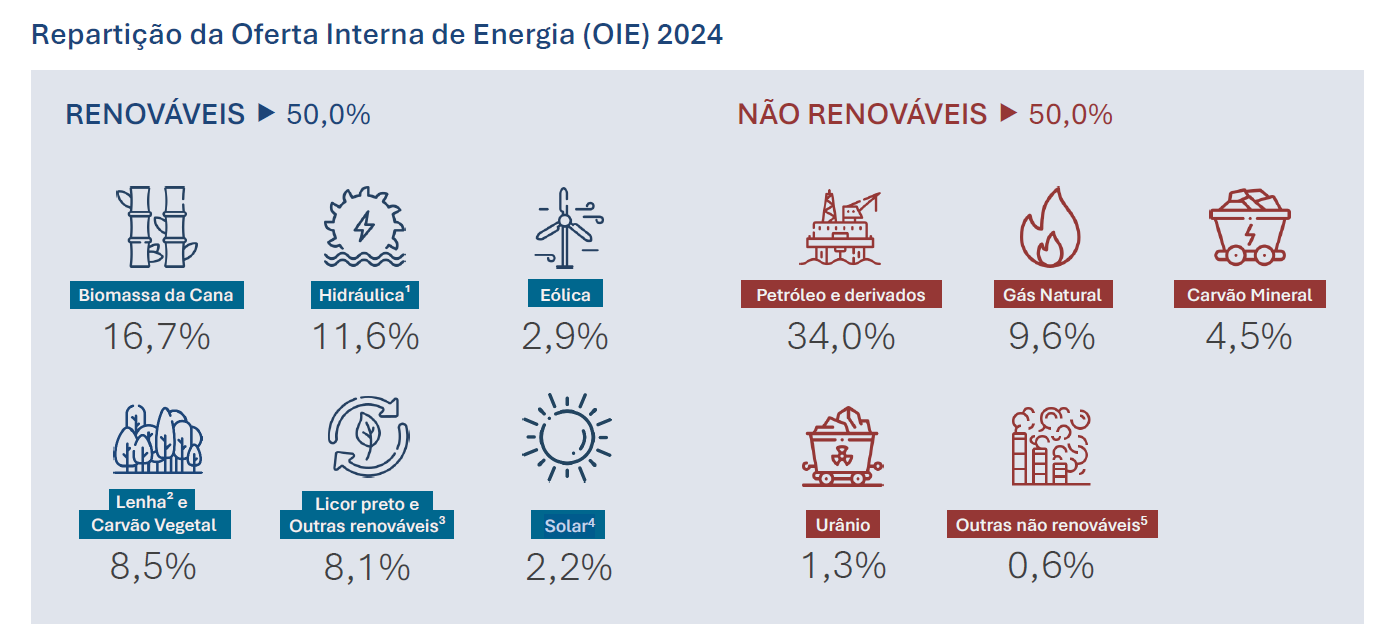
\includegraphics[width=0.65\linewidth]{figuras/introducao/dado_atuais/oie_2024.png}
    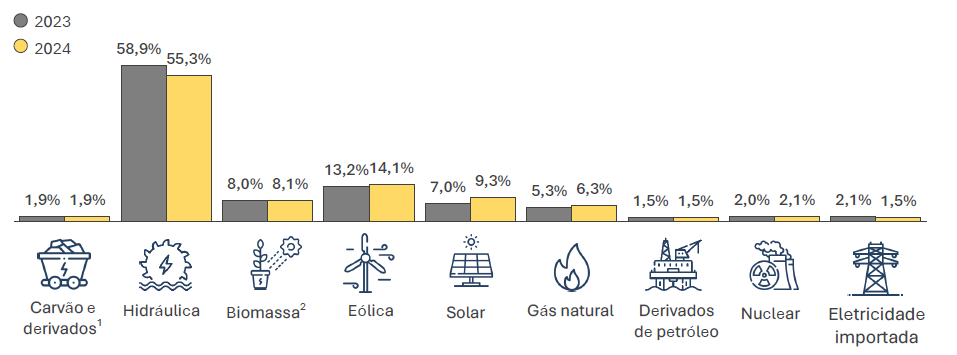
\includegraphics[width=0.65\linewidth]{figuras/introducao/dado_atuais/matriz_ele.png}
    \caption{De cima para abaixo: composição percentual da OIE para cada fonte de energia e composição percentual da matriz elétrica para cada fonte ambas para 2024.}
    \label{fig:placeholder}
    \legend{Fonte: \citeonline{EPE2025}.}
\end{figure}

Além disso, a energia fotovoltaica apresenta um elevado crescimento que torna-se evidente ao se analisar a série histórica. No âmbito da OIE, a participação da energia solar saltou de \SI{0,2}{\percent} em 2015 para \SI{2,2}{\percent} em 2024, configurando a fonte de maior crescimento
percentual no período \cite{EPE2025}. Esse avanço é impulsionado de forma expressiva pela micro e minigeração distribuída (MMGD), majoritariamente composta por sistemas fotovoltaicos, que já corresponde a cerca de \SI{5,6}{\percent} de toda a geração elétrica do país \cite{EPE2025}. Nesse sentido, os dados consolidados da evolução da participação das diferentes fontes na matriz elétrica e na OIE, são apresentados nas Figuras~\ref{fig:variacao-oie} e \ref{fig:matriz-eletrica}.

\newpage

\begin{figure}[!h]
    \centering
    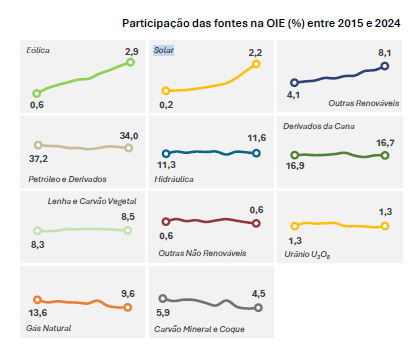
\includegraphics[width=0.5\linewidth]{figuras/introducao/dado_atuais/crescimento_fontes.png}
    \caption{Evolução temporal da participação de cada fonte de energia na OIE(\%) entre 2015 e 2024.}
    \legend{Fonte:\citeonline{EPE2025}}
    \label{fig:variacao-oie}
\end{figure}

\begin{figure}[!h]
    \centering
    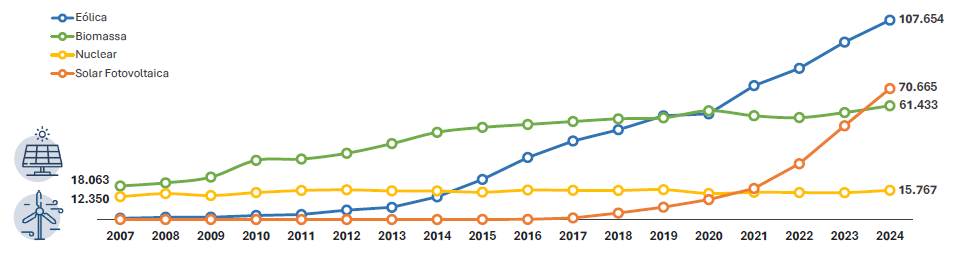
\includegraphics[width=0.9\linewidth]{figuras/introducao/dado_atuais/imagem_2026-05-31_204219085.png}
    \caption{Evolução da geração de energia elétrica por cada fonte.}
    \label{fig:matriz-eletrica}
    \legend{Fonte:\citeonline{EPE2025}}
\end{figure}

Dados mais recentes confirmam a continuidade dessa trajetória. Segundo a Associação Brasileira de Energia Solar Fotovoltaica, a capacidade fotovoltaica operacional no país superou \SI{70,3}{\giga\watt} em abril de 2026, considerando de forma agregada a geração centralizada e a distribuída \cite{absolar2026infografico}. Cabe observar que esse valor não é diretamente comparável aos \SI{48468}{\mega\watt} reportados pelo Balanço Energético Nacional, uma vez que se refere a uma data de corte posterior (abril de 2026, ante dezembro de 2024) e adota o critério metodológico do Ministério de Minas e Energia, que adiciona à capacidade instalada de cada fonte as parcelas associadas de micro e minigeração distribuída. Independentemente do critério, ambos os indicadores apontam para a mesma tendência de expansão acelerada.

Esse crescimento já produz efeitos sistêmicos relevantes. Em 26 de dezembro de 2025, a fonte solar atingiu o recorde de \SI{42552}{\mega\watt} de geração instantânea, equivalente a \SI{48,37}{\percent} da demanda nacional naquele momento; no mês de dezembro de 2025, respondeu por \SI{15,23}{\percent} de toda a oferta de energia elétrica do país \cite{absolar2026infografico}. Tal nível de penetração de uma fonte de caráter intermitente evidencia, contudo, os desafios operacionais associados à sua variabilidade, os quais serão retomados na Subseção~\ref{subsec:relevancia} como elemento central para a justificativa deste trabalho.

Dessa forma, os dados apresentados evidenciam que a energia fotovoltaica é uma fonte em ascensão, que em menos de uma década deixou de ser marginal para se tornar uma das protagonistas da expansão da matriz elétrica nacional. Esse desempenho expressivo, contudo, não decorre exclusivamente de incentivos regulatórios ou da redução de custos da tecnologia, mas encontra respaldo, sobretudo, nas condições físicas privilegiadas do território brasileiro para o aproveitamento da energia solar. Nesse sentido, para dimensionar adequadamente esse potencial e compreender o quanto dele ainda permanece inexplorado, faz-se necessário situar o Brasil no contexto internacional, comparando seus recursos e seu grau de aproveitamento com o de outros países.

\subsection{Comparação com outros países}
\label{subsec:comparacao_paises}

Apesar de expressiva, a expansão acelerada descrita na subseção anterior, ainda
representa uma fração modesta do potencial físico do território brasileiro. No entanto, para
dimensionar esse descompasso, é elucidativo confrontar o Brasil com duas das
maiores potências fotovoltaicas mundiais em capacidade instalada que é China e
Alemanha, distinguindo, primeiro, dois conceitos chaves: o
\emph{recurso solar disponível}, de natureza geográfica e climática, e o
\emph{grau de aproveitamento}, de natureza tecnológica,
econômica e regulatória. Os indicadores de recurso utilizados nesta comparação
provêm do estudo \textit{Global Photovoltaic Power Potential by Country}, produzido pelo
Banco Mundial em parceria com a Solargis \cite{WorldBank2020} e que padroniza,
para fins de comparabilidade entre países, a irradiação horizontal global
média (GHI, em \si{\kWh\per\square\metre\per\day}) como medida do potencial
teórico e a produtividade específica de uma usina de referência (PVOUT, em
\si{\kWh\per\kWp\day}) como medida do potencial prático.

\begin{figure}[!h]
    \centering
    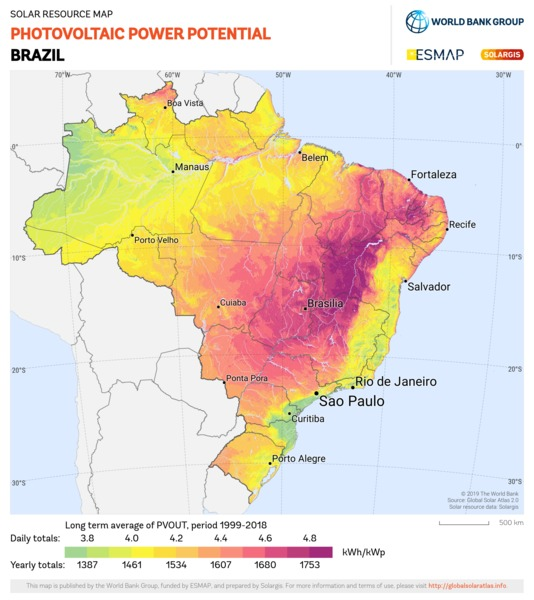
\includegraphics[width=0.3\linewidth]{figuras/introducao/comparacao/Brazil_PVOUT_mid-size-map_156x175mm-300dpi_v20191015.preview.jpg}
    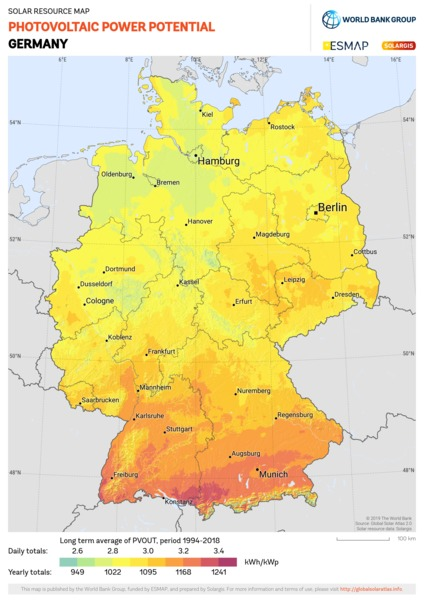
\includegraphics[width=0.3\linewidth]{figuras/introducao/comparacao/Germany_PVOUT_mid-size-map_156x220mm-300dpi_v20191205.preview.jpg}
    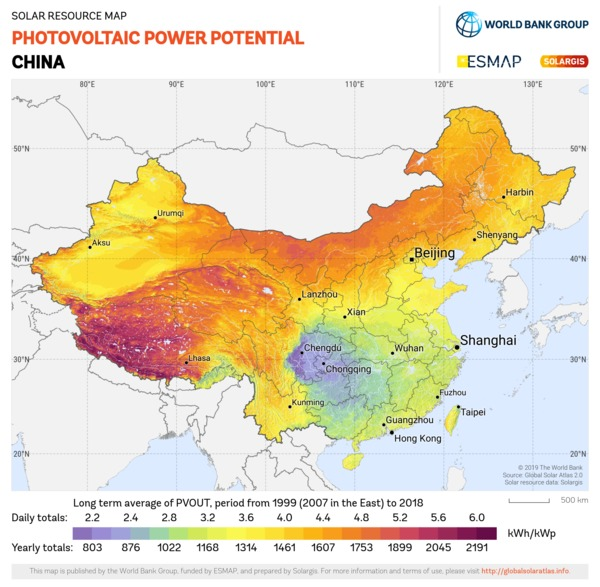
\includegraphics[width=0.3\linewidth]{figuras/introducao/comparacao/China_PVOUT_mid-size-map_156x152mm-300dpi_v20191015.preview.jpg}
    \caption{Mapas de produtividade fotovoltaica (PVOUT) do Brasil, Alemanha e China.}
    \label{fig:pvout-maps}
\end{figure}

A Alemanha é, historicamente, o país que pavimentou o mercado fotovoltaico
mundial, mas o faz a despeito de um recurso solar reconhecidamente escasso.
Segundo o estudo do Banco Mundial, o potencial teórico médio alemão é de apenas
\SI{2,978}{\kWh\per\square\metre\per\day} de GHI, ocupando a posição~197 no \textit{ranking}
mundial, ao passo que o Brasil registra \SI{5,276}{\kWh\per\square\metre\per\day},
ocupando a 89.\textsuperscript{a} posição \cite{WorldBank2020}. Em termos de
potencial prático, a produtividade média (PVOUT, nível~1) é de
\SI{2,961}{\kWh\per\kWp\per\day} na Alemanha contra
\SI{4,404}{\kWh\per\kWp\per\day} no Brasil \cite{WorldBank2020}. A diferença é
de tal ordem que o \textit{máximo} potencial prático observado em território
alemão (\SI{3,33}{\kWh\per\kWp\per\day}) é inferior ao \textit{mínimo}
registrado em qualquer ponto do território brasileiro
(\SI{3,75}{\kWh\per\kWp\per\day}) \cite{WorldBank2020}. Isto é, no
local menos ensolarado do Brasil é possível gerar mais eletricidade solar do
que no local mais ensolarado da Alemanha \cite{pereira2017atlas}. A esse maior
nível de irradiação soma-se uma vantagem qualitativa relevante para a operação
do sistema que é a baixa sazonalidade brasileira. Enquanto a razão entre o mês de
maior e o de menor produtividade (índice de sazonalidade) atinge $4{,}37$ na
Alemanha, no Brasil esse índice é de apenas $1{,}34$ \cite{WorldBank2020}, o que
se traduz em geração mais uniforme ao longo do ano e, portanto, em menor esforço
de balanço sazonal por parte do operador do sistema.

Apesar dessa inferioridade de recursos, a Alemanha mantém uma das maiores
bases instaladas do planeta, da ordem de \SI{117}{\giga\watt}, com adições
anuais médias próximas a \SI{19,6}{\giga\watt} \cite{BMWK2025}. Dessa forma, fica claro que o pioneirismo alemão decorreu não de condições naturais
favoráveis, mas de políticas de incentivo de longo prazo --- notadamente as
tarifas \textit{feed-in} ---, de maturidade industrial e de previsibilidade
regulatória. Essa constatação reforça que o aproveitamento da energia solar é
determinado tanto pelo recurso disponível quanto pelos arranjos
institucionais e tecnológicos que o viabilizam, dentre os quais se inclui a
capacidade de prever a geração com precisão, tema central deste trabalho.

Já a China apresenta um perfil intermediário no que tange ao recurso, mas é, em
larga margem, a líder absoluta em capacidade instalada. Seu potencial teórico
médio é de \SI{4,127}{\kWh\per\square\metre\day} de GHI (posição~161) e o
potencial prático médio, de \SI{3,883}{\kWh\per\kWp\day} de PVOUT
(posição~151) \cite{WorldBank2020}. Ambos os indicadores situam-se
significativamente abaixo dos valores brasileiros
(\SI{5,276}{\kWh\per\square\metre\per\day} e
\SI{4,404}{\kWh\per\kWp\day}, respectivamente), embora a heterogeneidade
territorial chinesa seja notável, o oeste do país, sobretudo o Deserto de Gobi e o Planalto Tibetano, exibem valores de PVOUT comparáveis aos melhores sítios brasileiros,
ao passo que as regiões orientais, mais populosas e industrializadas,
apresentam produtividade bastante inferior. Em relação a sazonalidade, o país apresenta um índice de $1{,}67$ \cite{WorldBank2020}, sendo superior à brasileira, porém, ainda que
mais favorável que a alemã.

No plano do aproveitamento, contudo, a assimetria se inverte de maneira
dramática. A China encerrou o período recente com capacidade fotovoltaica
instalada da ordem de \SI{1,23}{\tera\watt}, aproximadamente vinte vezes a
base instalada brasileira, além de ter um crescimento anual em torno de
\SI{33,2}{\percent} e com previsão de adição de \SIrange{180}{240}{\giga\watt}
ao longo de 2026 \cite{nea2026}. Apenas a expansão chinesa projetada para um
único ano supera, portanto, toda a capacidade fotovoltaica operacional no Brasil. O caso chinês evidencia uma faceta complementar à da Alemanha: trata-se de um país que não dispõe do melhor recurso solar, mas que, por meio de escala industrial, integração da cadeia produtiva e políticas de Estado, transformou a energia solar em pilar central de sua matriz elétrica.

A liderança chinesa, contudo, não se restringe à capacidade instalada em
território próprio, uma verz que o país consolidou-se também como o centro nevrálgico da
cadeia produtiva global de equipamentos fotovoltaicos. Em 2024, a China foi
responsável por \SI{93,2}{\percent} da produção mundial de polissilício,
\SI{96,6}{\percent} das lâminas (\textit{wafers}), \SI{92,3}{\percent} das
células fotovoltaicas e \SI{86,4}{\percent} dos módulos \cite{Davidson2026}.
Essa concentração, somada à escala de produção, pressionou os preços dos módulos
a mínimos históricos --- frequentemente abaixo de \SI{1}{RMB\per\watt} ---,
tornando-os economicamente inviáveis para fabricantes de outras regiões
\cite{Davidson2026}. Tal domínio reforça a constatação anterior de que o avanço
chinês na geração apoia-se em uma posição dominante sobre toda a cadeia de valor,
desde a matéria-prima até o produto final, o que situa o país não apenas como o
maior gerador, mas como o principal fornecedor mundial da tecnologia. Cabe
ressaltar, ainda, o vigor da expansão recente: somente em 2025 a China adicionou
cerca de \SI{315}{\giga\watt} de capacidade fotovoltaica \cite{PVMagazine2026},
montante que, isoladamente, supera várias vezes toda a capacidade instalada
acumulada pelo Brasil até o presente.

A Tabela~\ref{tab:comparacao_paises} consolida os principais indicadores
discutidos, contrastando o recurso solar disponível com o grau de
aproveitamento em cada país.

\begin{table}[htbp]
\centering
\caption{Comparativo de potencial solar, capacidade instalada e crescimento:
Brasil, China e Alemanha.}
\label{tab:comparacao_paises}
\begin{tabular}{lrrr}
\hline
\textbf{Indicador} & \textbf{Brasil} & \textbf{China} & \textbf{Alemanha} \\
\hline
\multicolumn{4}{l}{\textit{Recurso solar (longo prazo)\textsuperscript{a}}} \\
\hline
Potencial teórico --- GHI (kWh/m\textsuperscript{2}/dia) & 5,276 & 4,127 & 2,978 \\
\quad \textit{posição no ranking mundial}                & 89.\textsuperscript{o} & 161.\textsuperscript{o} & 197.\textsuperscript{o} \\
Potencial prático --- PVOUT (kWh/kWp/dia)                & 4,404 & 3,883 & 2,961 \\
\quad \textit{posição no ranking mundial}                & 84.\textsuperscript{o} & 151.\textsuperscript{o} & 197.\textsuperscript{o} \\
Índice de sazonalidade ($-$)                             & 1,34 & 1,67 & 4,37 \\
Área equivalente (\% do território)                      & 0,03\% & 0,46\% & 2,95\% \\
\hline
\multicolumn{4}{l}{\textit{Aproveitamento (dados recentes)\textsuperscript{b}}} \\
\hline
Capacidade instalada                                     & $\approx$70,3 GW & $\approx$1.230 GW & $\approx$117 GW \\
Adição/crescimento recente                               & +28,1\%/ano & +315 GW (2025) & +19,6 GW/ano \\
\hline
\end{tabular}
\legend{\textsuperscript{a}~Fonte: \citeonline{WorldBank2020}, referente ao
estudo \textit{Global Photovoltaic Power Potential by Country} (dados de longo
prazo, 2020). \\
\textsuperscript{b}~Capacidade do Brasil em abril de 2026
\cite{absolar2026infografico}; capacidade e crescimento da China
\cite{nea2026,PVMagazine2026}; capacidade e crescimento da Alemanha
\cite{bmwk2025}. O crescimento do Brasil refere-se à expansão da capacidade
instalada em 2024 sobre 2023 \cite{EPE2025}.}
\end{table}

A confrontação com Alemanha e China revela um quadro paradoxal. O Brasil reúne,
simultaneamente, um recurso solar superior ao desses dois países com uma maior
irradiação média e, sobretudo, uma menor sazonalidade, além de um grau de
aproveitamento ainda incipiente quando medido em termos relativos, isto é, a área
equivalente necessária para suprir todo o consumo elétrico nacional com geração
fotovoltaica é estimada em apenas \SI{0,03}{\percent} do território, contra
\SI{0,46}{\percent} da China e \SI{2,95}{\percent} da Alemanha
\cite{WorldBank2020}, um indicador que sintetiza a folga existente entre
potencial e exploração. Fica evidente, assim, que o gargalo brasileiro não
reside no recurso natural, mas na capacidade de integrar de forma eficiente e
confiável uma fonte de caráter intermitente a um sistema elétrico de dimensões
continentais. É precisamente nesse ponto que se insere a contribuição deste
trabalho uma previsão acurada da geração fotovoltaica constitui um elemento
habilitador para que o vasto potencial brasileiro --- particularmente o da
região Nordeste, abordado na subseção seguinte --- seja convertido em geração
efetiva e despachável, mitigando os efeitos de sua variabilidade sobre a
operação do sistema.

\subsection{Grande potencial ainda não totalmente aproveitado no Nordeste}
\label{subsec:potencial_nordeste}

A vantagem brasileira evidenciada na comparação internacional não se distribui
de modo homogêneo pelo território. Conforme atestado pela segunda edição do
\textit{Atlas Brasileiro de Energia Solar}, elaborado pelo Laboratório de
Modelagem e Estudos de Recursos Renováveis de Energia (LABREN) do Instituto
Nacional de Pesquisas Espaciais (INPE) a partir do modelo de transferência
radiativa BRASIL-SR, a região Nordeste concentra os maiores níveis de
irradiação solar do país \cite{Pereira2017}. Os mapas de irradiação global
horizontal (GHI) ali apresentados situam o semiárido nordestino, em especial o
interior da Bahia e o vale do São Francisco, na faixa de maior incidência da
escala nacional, com totais diários médios anuais que se aproximam do limite
superior observado no território, da ordem de \SI{6,5}{\kWh\per\square\metre\per\day}
\cite{Pereira2017}. Em termos de potencial prático, os dados do estudo
\textit{Global Photovoltaic Power Potential by Country} corroboram essa
constatação, enquanto a mediana brasileira de PVOUT é de
\SI{4,42}{\kWh\per\kWp\day}, o valor máximo registrado no país alcança
\SI{4,92}{\kWh\per\kWp\day}, patamar associado justamente às áreas do
Nordeste \cite{WorldBank2020}.

A esse recurso de elevada magnitude soma-se uma característica de grande
relevância para a operação de sistemas fotovoltaicos que é a baixa variabilidade
sazonal. O regime de irradiação do semiárido é marcado por reduzida cobertura
de nuvens e pequena oscilação ao longo do ano, o que confere à região um índice
de sazonalidade inferior ao da média nacional \cite{Pereira2017,WorldBank2020}.
Tal estabilidade é tecnicamente desejável, pois implica geração mais uniforme
entre as estações e, consequentemente, maior previsibilidade da produção
energética, um atributo que, como se discutirá adiante, é determinante para a
integração da fonte ao sistema elétrico.

Esse conjunto de fatores físicos explica a forte concentração da geração
centralizada na região. De acordo com o levantamento mais recente da
Associação Brasileira de Energia Solar Fotovoltaica, entre os estados com maior
capacidade fotovoltaica centralizada outorgada figuram, logo após Minas Gerais,
a Bahia (\SI{20293,1}{\mega\watt}), o Piauí (\SI{17388,1}{\mega\watt}), o Ceará
(\SI{14503,5}{\mega\watt}), o Rio Grande do Norte (\SI{9383,1}{\mega\watt}), a
Paraíba (\SI{4087,2}{\mega\watt}) e Pernambuco (\SI{3812,1}{\mega\watt})
\cite{absolar2026infografico}. Considerados em conjunto, os estados nordestinos
respondem pela maior parcela da capacidade centralizada do país, refletindo a
preferência dos empreendimentos de grande porte por sítios de elevada
produtividade.

Subsiste, contudo, um descompasso expressivo entre o recurso disponível e o
montante efetivamente convertido em geração, descompasso esse que tende a se
agravar à medida que a capacidade instalada cresce mais rapidamente do que a
infraestrutura de transmissão e os mecanismos de gestão da rede. Um indício
concreto desse limite operacional já em curso é o aumento dos cortes de geração
(\textit{curtailment}) impostos às usinas solares: segundo o Operador Nacional
do Sistema, as restrições de geração em usinas fotovoltaicas cresceram de forma
acentuada nos últimos anos, alcançando, em 2025, montante equivalente a cerca
de \SI{20,7}{\percent} da geração \cite{absolar2026infografico}. Em outras
palavras, parcela relevante da energia que a região é fisicamente capaz de
produzir deixa de ser injetada na rede, o que evidencia que o gargalo brasileiro
--- e nordestino em particular --- reside não na disponibilidade do recurso, mas
na capacidade de integrá-lo de forma confiável a um sistema elétrico de
dimensões continentais.

Para dimensionar a ordem de grandeza desse potencial, é elucidativo um exercício
de estimativa. Adotando-se a produtividade específica máxima reportada para o
território nacional pelo \textit{Global Photovoltaic Power Potential by Country},
de \SI{4,92}{\kWh\per\kWp\per\day} --- equivalente a aproximadamente
\SI{1796}{\kWh\per\kWp} ao ano \cite{WorldBank2020} --- e uma densidade de
potência instalada característica de usinas de grande porte com módulos fixos de
silício cristalino, situada na faixa de \SIrange{60}{75}{\watt\peak\per\square\metre}
quando contabilizado o espaçamento entre fileiras\footnote{A densidade de
potência considera a área total ocupada pela usina, incluindo o espaçamento
entre fileiras de módulos necessário para evitar sombreamento mútuo, e não
apenas a área ativa dos painéis. A produtividade específica refere-se a sistemas
fixos com módulos monofaciais de silício cristalino e inclinação ótima, conforme
a metodologia adotada em \citeonline{WorldBank2020}. Trata-se de uma estimativa
de ordem de grandeza, que não incorpora restrições de uso do solo, áreas de
preservação, disponibilidade hídrica ou limitações da infraestrutura de
transmissão.}, é possível estimar o potencial de geração associado à ocupação de
diferentes frações da área da região Nordeste, cuja extensão territorial é de
cerca de \SI{1,55e6}{\square\kilo\metre}.

Os resultados, sintetizados na Tabela~\ref{tab:potencial_nordeste}, evidenciam a
magnitude do recurso. A ocupação de apenas \SI{1}{\percent} do território
nordestino seria suficiente para gerar entre \num{1675} e \SI{2093}{\tera\watt\hour}
por ano, montante equivalente a cerca de \numrange{2,2}{2,8} vezes toda a energia
elétrica gerada no Brasil em 2024 (\SI{751}{\tera\watt\hour}). Caso a fração
considerada fosse de \SI{5}{\percent}, a geração teórica superaria em mais de dez
vezes a produção nacional atual. Tais valores não representam, evidentemente,
metas de implantação --- são fisicamente irrealizáveis em sua totalidade ---, mas
explicitam a folga existente entre o recurso disponível e seu aproveitamento, bem
como reforçam que a limitação ao avanço da fonte não é de natureza física, e sim
operacional e sistêmica.

\begin{table}[htbp]
\centering
\caption{Estimativa de ordem de grandeza do potencial de geração fotovoltaica do
Nordeste para diferentes frações de ocupação territorial.}
\label{tab:potencial_nordeste}
\begin{tabular}{lrrr}
\hline
\textbf{Fração da área} & \textbf{Densidade} & \textbf{Capacidade} & \textbf{Geração anual} \\
\textbf{do Nordeste}    & \textbf{(W$_p$/m\textsuperscript{2})} & \textbf{(GW$_p$)} & \textbf{(TWh/ano)} \\
\hline
\multirow{2}{*}{1\%} & 60 &   933 & 1.675 \\
                     & 75 & 1.166 & 2.093 \\
\hline
\multirow{2}{*}{5\%} & 60 & 4.663 &  8.374 \\
                     & 75 & 5.829 & 10.467 \\
\hline
\end{tabular}
\legend{Fonte: elaborado pelo autor a partir de \citeonline{WorldBank2020} e
\citeonline{EPE2025}. Premissas: PVOUT de \SI{4,92}{\kWh\per\kWp\per\day}
($\approx$\SI{1796}{\kWh\per\kWp\per\year}); área do Nordeste de
\SI{1,55e6}{\square\kilo\metre}. Comparação: geração elétrica total do Brasil em
2024 $=$ \SI{751}{\tera\watt\hour} \cite{EPE2025}.}
\end{table}

\subsection{Empecilhos para aproveitar o potencial}
\label{subsec:empecilhos}

A análise das subseções anteriores deixa claro que o gargalo brasileiro para a
expansão da geração fotovoltaica não reside na disponibilidade do recurso solar,
mas em um conjunto de fatores de natureza operacional, técnica e
institucional. A literatura especializada converge ao apontar que a distância
entre o potencial físico e o efetivamente convertido em geração decorre de
barreiras que extrapolam a dimensão econômica usualmente enfatizada
\cite{Fratea2017,Queiroz2020}. Dessa forma, discutem-se, nesta subseção, três desses
empecilhos: a capacidade limitada da infraestrutura de transmissão, a
escassez de mão de obra técnica qualificada e o ambiente tributário-regulatório, selecionados por sua relevância recorrente na literatura e por sua conexão
direta com a justificativa deste trabalho.

Entre as barreiras de caráter técnico, a insuficiência da rede de transmissão é
reiteradamente apontada como a mais crítica para a viabilização de
empreendimentos de grande porte. Nesse cenário, um estudo conduzido com agentes do setor
elétrico do estado de Minas Gerais, \citeonline{Fratea2017} identificaram, por
meio do método~Q, que a percepção de que ``a rede de transmissão de eletricidade
não dispõe de capacidade para escoar a eletricidade solar que a geração
fotovoltaica pode produzir'' figura entre as barreiras estatisticamente mais
significativas e mais bem ranqueadas pelos \emph{stakeholders}. Para esse grupo,
o gargalo de transmissão é considerado mais determinante do que o próprio preço
ofertado nos leilões, sob o argumento de que a elevada irradiação de um sítio é
condição necessária, mas não suficiente, à viabilidade do projeto: ``usinas
solares instaladas em locais de alta radiação não têm valor algum se não houver
meio de escoar a energia'' \cite{Fratea2017}. O mesmo estudo registra um caso
emblemático em que uma usina projetada para gerar \SI{2,78}{\mega\watt} de pico
estava limitada por uma capacidade local de rede de apenas \SI{1,25}{\mega\watt}
\cite{Fratea2017}, ilustrando o descasamento entre a capacidade de geração e a de
escoamento.

Esse diagnóstico, formulado em 2017, materializa-se hoje em um indicador
concreto e crescente que é o corte de geração (\textit{curtailment}). Conforme já
mencionado na Subseção~\ref{subsec:potencial_nordeste}, as restrições de geração
impostas às usinas fotovoltaicas pelo Operador Nacional do Sistema alcançaram,
em 2025, montante equivalente a cerca de \SI{20,7}{\percent} da geração total
\cite{absolar2026infografico}. Em outras palavras, a barreira de transmissão
deixou de ser uma projeção teórica e tornou-se uma perda mensurável de energia
já geráveis, agravada pelo fato de a expansão da capacidade instalada ocorrer em
ritmo superior ao da ampliação das linhas de transmissão.

Um segundo empecilho, de natureza estrutural, é a carência de profissionais
tecnicamente capacitados para sustentar o ciclo de vida dos sistemas
fotovoltaicos. \citeonline{Fratea2017} relatam forte concordância entre os
agentes do setor com a afirmação de que ``a ausência de mão de obra
especializada prejudica o desenvolvimento de usinas solares'', justificada pela
necessidade de capacidade técnica especializada ``desde a concepção do projeto
até a instalação, operação e manutenção''. Um dos entrevistados adverte, de
forma incisiva, que a falta de mão de obra qualificada ``resultará em falhas
operacionais, o que poderia favorecer tecnologias mais consolidadas, como a
hidreletricidade'' \cite{Fratea2017} --- observação particularmente relevante
para este trabalho, na medida em que falhas operacionais e a baixa qualidade
da operação comprometem diretamente a previsibilidade e a confiabilidade da
geração.

Essa lacuna é igualmente apontada como uma das limitações intrínsecas da fonte
em revisões da literatura, que listam a ``falta de especialistas para
manutenção, inspeção, reparo e avaliação'' entre as principais barreiras ao
aproveitamento da energia solar \cite{Queiroz2020}. A dimensão do
empecilho fica evidente no contraste internacional: na Alemanha, em 2013, o
setor de energias renováveis já empregava mais de \num{370000} trabalhadores em
empregos diretos, número que ultrapassava \num{1,5} milhão quando consideradas as
atividades de pesquisa, desenvolvimento, treinamento e educação associadas
\cite{Queiroz2020}. Cabe registrar, contudo, uma ressalva: parte da literatura
argumenta que essa barreira é mitigável no médio prazo, dada a existência, em
regiões de elevado potencial, de instituições de ensino técnico e superior
capazes de formar a mão de obra necessária localmente \cite{Fratea2017}. Trata-se,
portanto, de um empecilho real, porém endereçável por meio de políticas de
qualificação profissional.

O terceiro grupo de empecilhos relaciona-se ao arcabouço tributário e
regulatório. Por um lado, o marco regulatório foi historicamente o principal
catalisador da expansão da fonte no país: a Resolução Normativa
n.\textsuperscript{o}~482/2012 da Agência Nacional de Energia Elétrica (ANEEL),
ao regulamentar o sistema de compensação de energia da micro e minigeração
distribuída, e os leilões específicos para usinas fotovoltaicas conduzidos pelo
governo federal foram determinantes para o crescimento observado
\cite{Urbanetz2018}. Por outro lado, a própria literatura reconhece que a
maturidade de mercados consolidados decorreu de instrumentos de incentivo de
longo prazo --- como as tarifas \textit{feed-in} adotadas na Alemanha e na
Espanha --- combinados a reduções e isenções tributárias sobre equipamentos e
sobre o lucro das empresas atuantes no setor \cite{Fratea2017,Queiroz2020}.

No caso brasileiro, a carga tributária e os custos de capital ainda elevados
contribuem para que o custo de implantação supere o de países de referência: em
2013, enquanto o custo de instalação na Alemanha era da ordem de
\SI{1684}{\text{\euro}\per\kWp}, no Brasil situava-se entre \num{2000} e
\SI{3000}{\text{\euro}\per\kWp}, isto é, praticamente o dobro \cite{Queiroz2020}.
Soma-se a isso a instabilidade do ambiente regulatório, frequentemente
identificada como barreira política, uma vez que a incerteza quanto à
manutenção das regras de incentivo eleva o risco percebido pelo investidor e
inibe o aporte de capital no setor \cite{Queiroz2020,Fratea2017}. Análises
quantitativas das barreiras à expansão da fonte no país sugerem, inclusive, que
as barreiras de natureza política e de conhecimento exercem influência superior
à das barreiras estritamente financeiras, ambientais e sociais
\cite{Queiroz2020}, o que reforça a centralidade dos arranjos institucionais ---
e não apenas do custo da tecnologia --- na explicação do aproveitamento ainda
incipiente do potencial brasileiro.

Em suma, os três empecilhos discutidos compartilham uma característica comum:
nenhum deles decorre de limitações do recurso solar, e todos se intensificam à
medida que a participação de uma fonte intermitente cresce na matriz elétrica.
A capacidade de transmissão, a disponibilidade de mão de obra e a estabilidade
regulatória condicionam o quanto do potencial físico pode ser efetivamente
convertido em geração confiável e despachável. É nesse contexto que se insere a
contribuição deste trabalho, conforme se detalha na subseção seguinte.

\subsection{Conexão com o trabalho apresentado e sua relevância}
\label{subsec:relevancia}

As subseções anteriores estabeleceram dois fatos centrais, primeiro, o Brasil dispõe de um
recurso solar excepcional, particularmente no Nordeste, e, segundo, o aproveitamento desse
recurso não é limitado por sua disponibilidade física, mas por barreiras de
natureza operacional, técnica e institucional. Resta, portanto, articular de que
modo um modelo de previsão de geração contribui para a superação dessas barreiras, 
articulação que constitui a justificativa central deste trabalho.

Nesse sentido, o ponto de partida é uma reinterpretação da própria natureza do problema. A
intermitência da geração fotovoltaica, frequentemente tratada como uma limitação
física intrínseca da fonte, é mais adequadamente compreendida como um problema de
informação. Do ponto de vista da operação do sistema, a variabilidade da
irradiância, causada por nebulosidade, sazonalidade e pelo próprio ciclo diário por exemplo, 
só se converte em risco operacional na medida em que é desconhecida ou mal
estimada. O Operador Nacional do Sistema Elétrico (ONS) necessita
saber, com antecedência suficiente, quanto cada usina irá gerar para programar o
despacho complementar das demais fontes, dimensionar reservas e preservar o
equilíbrio entre geração e carga. Quando essa informação é imprecisa ou
indisponível, o operador é compelido a adotar uma postura conservadora, mantendo
reservas térmicas girantes em operação permanente para fazer frente a desvios
inesperados de geração. Tal solução é, simultaneamente, custosa, poluente e
prejudicial à competitividade econômica da própria fonte solar, na medida em que
parte de seu benefício ambiental e tarifário é anulada pela necessidade de
respaldo térmico contínuo.

Sob essa ótica, melhorar a acurácia da previsão de geração equivale a reduzir a
incerteza com que o operador trabalha e, por conseguinte, a margem de reserva que
precisa manter. \citeonline{Tian2023} quantificam esse efeito de forma direta, afirmando que
uma melhoria de \SI{25}{\percent} na acurácia da previsão de geração fotovoltaica
é capaz de reduzir o custo líquido de geração do sistema em \SI{1,56}{\percent},
o que equivale a cerca de US\$~46,5~milhões por ano no caso analisado. Dessa forma, a relação
evidencia que a previsão não é um exercício meramente acadêmico, mas um insumo
operacional com efeitos econômicos mensuráveis. Cada incremento de acurácia se
traduz em menor acionamento de reservas, menor custo de balanço e maior espaço
para a injeção efetiva da geração solar na rede.

Esse mecanismo conecta-se diretamente aos empecilhos discutidos na
Subseção~\ref{subsec:empecilhos}. O \textit{curtailment} crescente --- que
alcançou cerca de \SI{20,7}{\percent} da geração fotovoltaica em 2025
\cite{absolar2026infografico} --- decorre, em parte, da limitação física da
transmissão, mas também da dificuldade do operador em coordenar, em tempo hábil,
uma geração cuja trajetória não é conhecida com precisão suficiente. Uma previsão
mais acurada não amplia, por si só, a capacidade das linhas, mas permite uma
gestão mais eficiente da capacidade existente, antecipando rampas de geração,
otimizando o despacho hidrotérmico e reduzindo cortes motivados por margem de
segurança excessiva. 

A relevância desse aporte intensifica-se no contexto nordestino. Conforme
discutido na Subseção~\ref{subsec:potencial_nordeste}, a região concentra a maior
parcela da capacidade fotovoltaica centralizada do país e opera em estreita
complementaridade com o parque hidrelétrico, cujos reservatórios são recorrentemente
pressionados pelas secas cíclicas do semiárido. Nesse contexto, erros de previsão
da geração solar propagam-se para o planejamento do despacho hidrotérmico, em que uma
superestimação da geração fotovoltaica pode levar ao deplecionamento desnecessário
de reservatórios, ao passo que uma subestimação implica acionamento térmico
evitável. A precisão da previsão adquire, portanto, um valor sistêmico que extrapola
a usina individual, condicionando a eficiência da operação integrada do
subsistema.

A relevância da previsão, contudo, não se restringe à perspectiva do operador
central. Do ponto de vista da iniciativa privada, como agentes geradores,
comercializadores e investidores em ativos fotovoltaicos, a acurácia da
previsão de geração incide diretamente sobre a receita e sobre a gestão do
negócio. No ambiente de comercialização, o gerador precisa programar
antecipadamente a energia que injetará na rede, e desvios entre a geração
programada e a efetivamente realizada estão sujeitos a mecanismos de liquidação
de diferenças que penalizam tanto a subentrega quanto a sobreentrega. Uma
previsão mais acurada reduz a magnitude desses desvios e, por conseguinte, a
exposição do agente a penalidades e à volatilidade do mercado de curto prazo,
estabilizando o fluxo de receita do empreendimento.

Para além da dimensão comercial, a previsão qualifica o planejamento operacional
do ativo. O conhecimento antecipado do perfil de geração subsidia o agendamento
de paradas para manutenção em janelas de baixa produtividade, a operação
coordenada com sistemas de armazenamento por baterias, cuja viabilidade
econômica depende de uma estratégia de carga e descarga informada pela geração
esperada, e a própria detecção de anomalias, na medida em que desvios
sistemáticos entre a geração prevista e a observada podem sinalizar
\textit{soiling}, sombreamento ou falhas de equipamento. 

Por fim, no horizonte do planejamento de longo prazo, modelos de previsão confiáveis reduzem a incerteza
sobre a produção esperada e, com ela, o risco percebido pelo investidor, fator
que --- como discutido na Subseção~\ref{subsec:empecilhos} --- influencia
diretamente o custo de capital e a atratividade dos empreendimentos
fotovoltaicos. Há, portanto, uma convergência de interesses, na qual a informação que
torna a operação do sistema mais eficiente e barata para o operador é a mesma que
melhora a previsibilidade financeira e a competitividade do gerador privado.

Em suma, este trabalho não se limita a desenvolver um modelo preditivo: ele
produz a informação de que o operador do sistema necessita, mas que ainda não
dispõe com a qualidade adequada às especificidades do contexto brasileiro. 
É esse deslocamento, de um problema percebido como físico para um problema de informação tratável por meio de modelagem, que confere
ao trabalho aplicação operacional concreta. Estando, dessa maneira, delimitado o problema e justificada
sua relevância, resta enunciar os objetivos que orientam a investigação.

\section{Objetivo do trabalho}
\label{subsec:objetivo}
% TODO: declarar objetivo geral e objetivos específicos do TG na sequência
% (ou remeter à Seção de Objetivos, conforme a estrutura adotada).

\section{Estrutura do texto}
\label{subsec:estrutura}

% !TeX root = ../main.tex
% ============================================================
%  Capítulo 2 – Referencial Teórico
% ============================================================
\chapter{Referencial Teórico}
\label{cap:referencial_teorico}

% ============================================================
\section{Previsão de Geração de Energia Fotovoltaica}
\label{sec:previsao_fv}
% ------------------------------------------------------------

\subsection{Especificidades para sistemas fotovoltaicos}
\label{subsec:especificidades_fv}

% TODO: Tratar sazonalidade diária e anual, ausência de geração noturna,
%       impacto de nuvens e aerossóis. Discutir normalização pela irradiância
%       (clear-sky index) como estratégia comum na literatura.

% ============================================================

A série temporal de geração de energia de uma usina fotovoltaica não constitui um sinal
arbitrário: ela resulta da modulação de uma forçante astronômica determinística, a
trajetória solar, por um conjunto de fatores atmosféricos de natureza estocástica. Dessa
dupla origem decorre um conjunto de propriedades estatísticas particulares que distinguem o
problema da previsão fotovoltaica de outras tarefas de previsão de séries temporais e que
condicionam diretamente as escolhas de modelagem, de engenharia de \emph{features} e de
validação adotadas neste trabalho. Esta subseção discute quatro dessas especificidades.

A geração fotovoltaica exibe forte autocorrelação, isto é, dependência estatística entre
valores da série separados por um intervalo de tempo. Em escalas curtas, essa dependência
é elevada e decai monotonicamente com a defasagem, instantes consecutivos apresentam
condições de irradiância e de carga muito semelhantes, de modo que a potência em um dado
instante é fortemente preditiva da potência nos instantes imediatamente seguintes
\cite{Zhou2022}. Essa propriedade é precisamente o que viabiliza as abordagens orientadas
por dados, e fundamenta a construção de preditores baseados em defasagens (\emph{lags}) e em médias móveis da série, que reintroduzem explicitamente essa memória temporal no vetor de entrada dos modelos. Importante salientar, contudo, que a autocorrelação não se restringe a defasagens curtas e dependendo do horizonte escolhido pode ser utilizado defasagens de mais de 24 horas.

A característica mais marcante da série de geração fotovoltaica é a presença de
sazonalidade múltipla, ou seja, a superposição de ciclos periódicos de diferentes
frequências. Dois ciclos predominam. O primeiro é o ciclo diário no qual a geração segue,
a cada dia, um perfil aproximadamente em forma de sino, nulo durante a noite, crescente
após o nascer do Sol, máximo ao redor do meio-dia solar e decrescente até o pôr do Sol. O
segundo é o ciclo anual, a amplitude e a duração desse perfil diário variam ao longo
do ano, em função da declinação solar e dos regimes sazonais de nebulosidade. A
manifestação conjunta dessas periodicidades é diretamente observável na distribuição
temporal do erro dos modelos de previsão, que tende a ser maior nas horas centrais do dia e
nos meses de maior irradiância, justamente onde a magnitude da geração é mais elevada
\cite{Kappler2024}. Essa estrutura sazonal determinística é, em grande medida, conhecida a
priori e pode ser fornecida ao modelo por meio de variáveis astronômicas, como elevação,
azimute e declinação solar, conforme adotado neste trabalho.

A potência gerada é uma grandeza fisicamente não-negativa e limitada superiormente
pela capacidade nominal da usina. Mais relevante do ponto de vista estatístico é o
fenômeno do truncamento diurno, ou seja, durante o período noturno, a geração é
identicamente nula, o que faz com que uma fração substancial das observações da série
assuma exatamente o valor zero, consequentemente, esse efeito distorce a distribuição da variável-alvo, tornando-a fortemente assimétrica e concentrada em zero, a ponto de que a mediana das
observações pode situar-se próxima de zero quando as amostras noturnas são contabilizadas
\cite{Andrade2023}. Tal característica tem duas implicações metodológicas. A primeira diz
respeito ao pré-processamento, no qual parte da literatura opta por remover as observações noturnas do conjunto de dados, tornando a série resultante mais homogênea e estacionária
\cite{Khalyasmaa2020}, enquanto outra parte as preserva, sob o argumento de que o modelo deve operar também nessas condições no cotidiano \cite{Andrade2023}. A segunda implicação refere-se à
própria saída do modelo na qual previsões fisicamente inconsistentes, como valores negativos ou
geração noturna não nula, devem ser tratadas, seja por truncamento explícito a zero, seja
pela imposição de limites dependentes do tempo derivados da geometria solar
\cite{Markovics2022}.

Por fim, a série de geração fotovoltaica é não-estacionária: suas propriedades
estatísticas, como média, variância e estrutura de autocorrelação, não permanecem constantes
ao longo do tempo. Parte dessa não-estacionariedade é determinística e decorre das próprias
sazonalidades já descritas, sendo, portanto, previsível. Outra parte, contudo, é induzida
por fatores externos de evolução lenta ou abrupta, tais como a degradação progressiva dos
módulos, o acúmulo de sujidade (\emph{soiling}) sobre as superfícies, o sombreamento
sazonal por obstáculos, falhas de equipamento e intervenções de manutenção. Esses fatores
alteram a relação entre a forçante meteorológica e a potência efetivamente gerada,
introduzindo mudanças no regime da série que não são explicáveis apenas pelas variáveis de
entrada. Do ponto de vista da modelagem, a não-estacionariedade impõe cautela, uma vez que um modelo ajustado a um período pode degradar seu desempenho quando aplicado a um período posterior
de regime distinto, o que reforça a necessidade de procedimentos de validação que
respeitem a ordem cronológica dos dados — tema retomado na
Subseção~\ref{subsec:cross_validation}.

Em síntese, a previsão de geração fotovoltaica é um problema de série temporal de natureza
particular, no qual uma estrutura determinística forte e conhecível, os ciclos solares,
coexiste com uma componente estocástica e não-estacionária das condições atmosféricas e do
estado das usinas. Dessa maneira, as decisões metodológicas adotadas neste trabalho, da seleção
de variáveis à estratégia de validação, pode ser compreendida como uma resposta direta a
essas quatro especificidades.

\subsection{Diferentes métodos de previsão}
\label{subsec:metodos_previsao}

% TODO: Classificar os métodos existentes: físicos/NWP, estatísticos (ARIMA etc.),
%       baseados em imagens de satélite/céu e baseados em ML/DL.
%       Discutir vantagens e limitações de cada abordagem.
%       Referências-chave: \citep{Antonanzas2016}, \citep{Voyant2017}.

% ------------------------------------------------------------

A literatura especializada propõe diferentes taxonomias para organizar os métodos
de previsão de geração fotovoltaica. Uma classificação recorrente, adotada por
\citeonline{Andrade2023}, distingue quatro classes: métodos físicos, estatísticos, de
inteligência artificial e híbridos. Neste trabalho, contudo, adota-se a partição mais
parcimoniosa proposta por \cite{Markovics2022}, na qual as abordagens de
inteligência artificial são compreendidas como um subconjunto das estatísticas,
resultando em três categorias: físicas, estatísticas e híbridas.
Essa escolha decorre do fato de que tanto os modelos estatísticos clássicos quanto os
de aprendizado de máquina compartilham a característica essencial de serem orientados
por dados (\textit{data-driven}), o que justifica seu agrupamento sob uma mesma categoria
conceitual.

Antes de detalhar cada classe, convém estabelecer a notação comum. Seja $\hat{P}_{ac}(t+h)$
a previsão da potência elétrica em corrente alternada gerada pela usina no instante
$t+h$, em que $t$ é o instante de emissão da previsão e $h$ o horizonte de previsão.
As abordagens distinguem-se, essencialmente, pela forma como modelam o mapeamento entre
as variáveis disponíveis no instante $t$ e essa grandeza-alvo.

Os métodos físicos baseiam-se em cadeias de modelos (\textit{model chains}) que descrevem
analiticamente os processos envolvidos na conversão da energia solar em energia elétrica
\cite{Markovics2022}. A entrada da cadeia é a irradiância prevista por modelos de
Previsão Numérica do Tempo (\textit{Numerical Weather Prediction} --- NWP) ou estimada a
partir de imagens de satélite \cite{Andrade2023}. Por essa razão, a abordagem é também
denominada indireta, pois a potência é obtida pela composição sucessiva de
submodelos, e não diretamente a partir de dados de operação \cite{Markovics2022}.

Formalmente, a cadeia pode ser representada como uma composição de funções
\begin{equation}
    \hat{P}_{ac} = (f_{\mathrm{conv}} \circ f_{\mathrm{trans}} \circ f_{\mathrm{sep}})(G_{h}, \boldsymbol{\theta}),
    \label{eq:model_chain}
\end{equation}
em que $G_{h}$ é a irradiância horizontal global (GHI) prevista e $\boldsymbol{\theta}$
reúne os parâmetros de projeto da usina, como orientação, inclinação, potência nominal e
coeficientes do módulo. Cada operador corresponde a uma etapa física:

\begin{enumerate}
    \item \textbf{Separação das componentes} ($f_{\mathrm{sep}}$): decompõe a GHI em suas
    parcelas direta normal ($G_{b}$) e difusa ($G_{d}$), uma vez que apenas a GHI costuma
    estar disponível. Modelos de separação estimam a fração difusa $k_{d} = G_{d}/G_{h}$
    como função do índice de claridade $k_{t} = G_{h}/G_{0}$, sendo $G_{0}$ a irradiância
    extraterrestre no plano horizontal \cite{Markovics2022}.

    \item \textbf{Transposição para o plano inclinado} ($f_{\mathrm{trans}}$): converte as
    componentes no plano horizontal para a irradiância no plano dos módulos ($G_{t}$),
    geralmente segundo
    \begin{equation}
        G_{t} = G_{b}\cos\theta_{i} + G_{d}\,R_{d} + \rho\,G_{h}\,R_{r},
        \label{eq:transposicao}
    \end{equation}
    em que $\theta_{i}$ é o ângulo de incidência, $R_{d}$ e $R_{r}$ são os fatores de
    transposição das componentes difusa e refletida, e $\rho$ é o albedo do solo.

    \item \textbf{Conversão irradiância-potência} ($f_{\mathrm{conv}}$): modela a eficiência
    do sistema, incorporando o efeito da temperatura de operação. Uma forma usual é
    \begin{equation}
        P_{ac} = \eta_{\mathrm{inv}}\,P_{\mathrm{nom}}\,\frac{G_{t}}{G_{\mathrm{STC}}}
        \left[1 + \gamma\,(T_{mod} - T_{\mathrm{STC}})\right],
        \label{eq:conversao}
    \end{equation}
    em que $P_{\mathrm{nom}}$ é a potência nominal, $G_{\mathrm{STC}} = 1000~\mathrm{W/m^2}$
    e $T_{\mathrm{STC}} = 25~^{\circ}\mathrm{C}$ são as condições-padrão de ensaio (STC),
    $\gamma < 0$ é o coeficiente de temperatura de potência, $\eta_{\mathrm{inv}}$ a
    eficiência do inversor, e a temperatura do módulo $T_{mod}$ é estimada a partir de
    $T_{amb}$, $G_{t}$ e da velocidade do vento por correlações empíricas, e.g.,
    $T_{mod} = T_{amb} + (G_{t}/G_{\mathrm{ref}})\,(T_{\mathrm{NOCT}} - 20)$
    \cite{Sohani2022}.
\end{enumerate}

Em aplicações de maior fidelidade, $f_{\mathrm{conv}}$ pode substituir a
Equação~\eqref{eq:conversao} por um modelo eletricamente fundamentado do módulo, como o
modelo de diodo único, cuja relação corrente-tensão é dada por
\begin{equation}
    I = I_{ph} - I_{0}\left[\exp\!\left(\frac{V + I R_{s}}{n V_{t}}\right) - 1\right]
    - \frac{V + I R_{s}}{R_{p}},
    \label{eq:diodo}
\end{equation}
em que $I_{ph}$ é a fotocorrente (proporcional a $G_{t}$), $I_{0}$ a corrente de saturação,
$V_{t}$ a tensão térmica, $n$ o fator de idealidade, e $R_{s}$, $R_{p}$ as resistências
série e paralela \cite{Sohani2022}.

A principal vantagem dessa abordagem é não exigir dados históricos de operação, já que
descreve o comportamento da usina a partir de seus parâmetros de projeto, os modelos
físicos, portanto, podem ser implementados antes mesmo de a usina entrar em operação
\cite{Andrade2023}. Em contrapartida, apresentam, em geral, acurácia inferior à dos métodos
orientados por dados e demandam conhecimento detalhado das especificações da planta
\cite{Markovics2022,Andrade2023}. Adicionalmente, a seleção dos submodelos que compõem cada
elo da cadeia (separação, transposição e conversão) exerce impacto considerável sobre a
acurácia final \cite{Markovics2022}, e os erros de cada etapa propagam-se ao longo da
composição da Equação~\eqref{eq:model_chain}.

Já os métodos estatísticos abrangem toda a gama de abordagens orientadas por dados, desde os
modelos estatísticos clássicos até as técnicas de aprendizado de máquina
\cite{Markovics2022}. O traço comum é estimar, a partir de um conjunto de dados históricos
$\{(\mathbf{x}_{i}, y_{i})\}_{i=1}^{N}$, uma função $\hat{f}$ que minimize uma função de
perda $\mathcal{L}$ sobre esses dados,
\begin{equation}
    \hat{f} = \arg\min_{f \in \mathcal{F}} \frac{1}{N}\sum_{i=1}^{N}
    \mathcal{L}\big(y_{i}, f(\mathbf{x}_{i})\big),
    \label{eq:erm}
\end{equation}
sendo $\mathcal{F}$ a classe de funções admissíveis e, tipicamente, $\mathcal{L}$ o erro
quadrático $\mathcal{L}(y,\hat{y}) = (y-\hat{y})^{2}$. A potência prevista é então
$\hat{P}_{ac}(t+h) = \hat{f}(\mathbf{x}_{t})$.

Os modelos diferenciam-se pela natureza do vetor de entrada $\mathbf{x}_{t}$ e pela classe
$\mathcal{F}$. Nos modelos autorregressivos clássicos, como os da família ARIMA, a
entrada é constituída pelos próprios valores passados da série de geração e dos erros
passados. Um modelo ARMA($p,q$), por exemplo, assume
\begin{equation}
    y_{t} = c + \sum_{i=1}^{p}\phi_{i}\,y_{t-i}
    + \sum_{j=1}^{q}\vartheta_{j}\,\varepsilon_{t-j} + \varepsilon_{t},
    \label{eq:arma}
\end{equation}
em que $\phi_{i}$ e $\vartheta_{j}$ são, respectivamente, os coeficientes autorregressivos
e de média móvel, e $\varepsilon_{t}$ é um ruído branco \cite{Andrade2023}. Dessa forma, esses modelos
são capazes de capturar dependências lineares na estrutura temporal da série, mas têm capacidade limitada
de representar as relações fortemente não lineares entre as variáveis meteorológicas e a
potência gerada.

Já os modelos de aprendizado de máquina (\textit{machine learning}) ampliam a classe $\mathcal{F}$ para famílias
não lineares e admitem como entrada um vetor de variáveis exógenas $\mathbf{x}_{t}$, como
irradiância, temperatura ambiente, velocidade do vento e ângulos solares.
Exemplos comuns na literatura de previsão fotovoltaica incluem máquinas de vetores de
suporte (\emph{Support Vector Machines}, SVM), florestas aleatórias (\emph{Random Forests}) e
redes neurais artificiais \cite{Andrade2023}. 

A principal vantagem operacional dos métodos estatísticos reside em não requererem
conhecimento dos parâmetros de projeto da usina, o que facilita sua implementação
\cite{Markovics2022}, sendo, dessa maneira, um atributo particularmente relevante para operadores que não dispõem
das especificações de parques distribuídos. Entre eles, as técnicas de aprendizado de
máquina são as mais empregadas \cite{Markovics2022} e, embora frequentemente apresentem os
melhores resultados, costumam exigir maior esforço computacional \cite{Andrade2023}. Como
limitações, herdam a dependência da quantidade e da qualidade dos dados de treinamento e
estão sujeitas a sobreajuste (\emph{overfitting}) quando a complexidade de $\mathcal{F}$
não é adequadamente regularizada.

Por último, os métodos híbridos combinam elementos físicos e estatísticos em diferentes configurações,
constituindo uma categoria abrangente que se refere à hibridização de quaisquer duas ou
mais abordagens das classes anteriores \cite{Markovics2022,Andrade2023}. Um exemplo
representativo é o pré-processamento físico da irradiância prevista por modelos NWP como
variável de entrada para um modelo de aprendizado de máquina. Nesse arranjo, a etapa física
fornece uma estimativa fisicamente consistente da irradiância no plano dos módulos, $G_{t}$,
e o modelo estatístico assume a conversão irradiância-potência, isto é,
\begin{equation}
    \hat{P}_{ac}(t+h) = \hat{f}\big(f_{\mathrm{trans}}(f_{\mathrm{sep}}(G_{h})),
    T_{amb}, V_{w}, \dots\big),
    \label{eq:hibrido}
\end{equation}
substituindo a conversão analítica das Equações~\eqref{eq:conversao}--\eqref{eq:diodo} por
um mapeamento aprendido dos dados.

Nesse cenário, a motivação é explorar a complementaridade entre as abordagens. \citeonline{Markovics2022}
verificam que a incorporação, ao conjunto de preditores de um modelo de aprendizado de
máquina, de variáveis calculadas analiticamente, como os ângulos de posição do Sol
(elevação, azimute e declinação), aprimoram de forma significativa a acurácia das previsões
de potência. Esse resultado evidencia que a fronteira entre as categorias é, na prática,
permeável, e sugere que a engenharia de \emph{features} de base física constitui uma forma
de hibridização de baixo custo e elevado retorno.

\subsection{Horizontes temporais de previsão}
\label{subsec:horizontes_temporais}

% TODO: Definir os horizontes: very short-term (< 1 h), short-term (1–48 h),
%       medium-term (dias) e long-term (semanas/meses).
%       Relacionar cada horizonte com as necessidades do operador de rede.

% ------------------------------------------------------------

A previsão de geração fotovoltaica não constitui um problema único, mas uma família de
problemas cujas variáveis de entrada relevantes, técnicas adequadas e
aplicações de destino variam acentuadamente conforme o horizonte de previsão
considerado, isto é, o intervalo de tempo entre o instante de emissão da previsão e o
instante previsto. Conforme observam \citeonline{Tian2023}, os valores de irradiância e
de potência mantêm forte relação com a escala temporal, de modo que a definição do
horizonte condiciona toda a estratégia de modelagem. A partir desse contexto, esta subseção apresenta, de forma
comparativa, as principais faixas de horizonte usualmente distinguidas na literatura,
situando ao final a opção adotada neste trabalho.

Com efeito, embora não exista uma fronteira universalmente padronizada entre as faixas, a literatura
converge para uma divisão em quatro classes, sendo elas a previsão de altíssimo curto prazo
(\emph{nowcasting} ou intra-hora), a de curto prazo (intra-dia), a de um dia à frente
(\emph{day-ahead}) e a de médio a longo prazo. O traço que melhor as distingue não é apenas
a duração, mas a natureza física dominante da incerteza em cada escala e, por
consequência, a fonte de informação mais adequada para reduzi-la.

\subsubsection*{Altíssimo curto prazo (nowcasting)}

Nessa faixa, que abrange de segundos a aproximadamente uma hora à frente, a variabilidade
da geração é governada quase exclusivamente pelo movimento de nuvens, que provoca rampas
abruptas de irradiância em escala de segundos a minutos. Dessa maneira, as técnicas mais eficazes são as
que capturam o estado instantâneo do céu, como imageadores de céu total (\emph{sky imagers}),
que extraem vetores de movimento de nuvens (\emph{cloud motion vectors}) a partir de
imagens hemisféricas, e modelos puramente autorregressivos baseados em medições de alta
frequência da própria usina \cite{Tian2023}. Além disso, modelos de Previsão Numérica do Tempo (NWP),
são inadequados nessa escala por sua resolução temporal e latência de processamento. As
aplicações típicas incluem o controle em tempo real de inversores, a gestão de rampas e a
operação coordenada com sistemas de armazenamento por baterias.

\subsubsection*{Curto prazo (intra-dia)}

Estendendo-se de aproximadamente uma hora a seis horas à frente, essa faixa caracteriza-se, especialmente,
pela transição entre o regime dominado por nuvens e aquele dominado pela dinâmica
atmosférica de meso-escala. As abordagens mais empregadas combinam a extrapolação de
imagens de satélite que oferecem cobertura espacial superior à dos imageadores de solo
com modelos estatísticos e de aprendizado de máquina alimentados por séries temporais
recentes \cite{Tian2023}. As aplicações estão associadas ao despacho intra-dia, ao
mercado de curto prazo e ao balanceamento operacional do sistema.

\subsubsection*{Um dia à frente (day-ahead)}

A previsão \emph{day-ahead}, comumente entendida como o horizonte de 24 a 48 horas à
frente, é a de maior relevância para a operação e a comercialização de energia, pois é a
escala em que tipicamente se programa o despacho do dia seguinte e se submetem as ofertas
ao mercado \cite{Markovics2022}. Nessa faixa, o movimento individual de nuvens já não é
previsível de forma determinística, o que conduz a duas estratégias distintas quanto à
informação utilizada. A primeira recorre à Previsão Numérica do Tempo (NWP), cujas
previsões de irradiância e demais variáveis meteorológicas para o dia seguinte alimentam
modelos de conversão irradiância-potência \cite{Markovics2022}. A segunda, de natureza
puramente endógena, dispensa qualquer informação meteorológica futura e projeta a geração
do dia seguinte exclusivamente a partir do histórico de geração e das variáveis medidas na
própria usina até o instante de emissão da previsão, explorando a estrutura de
autocorrelação e os padrões diários e sazonais da série temporal. Diversos estudos da
literatura adotam essa segunda estratégia, utilizando como preditores a potência gerada e
as variáveis meteorológicas observadas em períodos anteriores \cite{Andrade2023}.

A abordagem endógena apresenta a vantagem prática de não requerer acesso a previsões NWP ao custo de uma acurácia tipicamente inferior à da abordagem
baseada em NWP, uma vez que se abstém da principal fonte de informação sobre as condições
atmosféricas futuras. Trata-se, portanto, de um compromisso entre disponibilidade de dados
e desempenho preditivo.

\subsubsection*{Médio e longo prazo}

Para horizontes que vão de alguns dias a meses ou anos, a previsibilidade da geração em um
instante específico essencialmente se perde, e o objeto da previsão desloca-se de valores
instantâneos para grandezas agregadas como médias diárias, mensais, sazonais ou anuais
\cite{Tian2023}. Predomina aqui a chamada previsão generalizada, na qual cada
conjunto de entradas corresponde a um valor agregado de saída \cite{Tian2023}. As
aplicações típicas situam-se no planejamento energético, no dimensionamento de ativos e na
estimativa de produção de longo prazo para fins de análise de viabilidade.

\subsubsection*{Síntese comparativa}

A Tabela~\ref{tab:horizontes} sintetiza as quatro faixas discutidas, contrastando o
horizonte, a fonte física dominante da variabilidade, as técnicas predominantes e as
principais aplicações.

\begin{table}[htb]
    \centering
    \caption{Comparativo das faixas de horizonte temporal de previsão de geração fotovoltaica.}
    \label{tab:horizontes}
    \begin{tabular}{p{2.4cm} p{2.0cm} p{3.4cm} p{3.2cm}}
        \toprule
        \textbf{Faixa} & \textbf{Horizonte típico} & \textbf{Técnicas predominantes} & \textbf{Aplicações principais} \\
        \midrule
        Altíssimo curto prazo (\emph{nowcasting}) & Segundos a $\sim$1\,h &
        Imageadores de céu total, vetores de movimento de nuvens, modelos autorregressivos &
        Controle de inversores, gestão de rampas, operação de baterias \\
        \addlinespace
        Curto prazo (intra-dia) & $\sim$1\,h a 6\,h &
        Extrapolação de imagens de satélite, aprendizado de máquina &
        Despacho intra-dia, mercado de curto prazo, balanceamento \\
        \addlinespace
        Um dia à frente (\emph{day-ahead}) & 24\,h a 48\,h &
        NWP acoplado a modelos de aprendizado de máquina, ou modelos puramente endógenos sobre séries históricas &
        Programação do despacho, comercialização no mercado diário \\
        \addlinespace
        Médio e longo prazo & Dias a anos &
        NWP de longo alcance, modelos climatológicos, previsão generalizada &
        Planejamento energético, dimensionamento de ativos, análise de viabilidade \\
        \bottomrule
    \end{tabular}
    \begin{flushleft}
    \footnotesize Fonte: elaborado pelo autor a partir de \citeonline{Markovics2022} e \citeonline{Tian2023}.
    \end{flushleft}
\end{table}

A delimitação dessas faixas permite situar com precisão o escopo deste trabalho, que se
concentra no horizonte de \emph{um dia à frente} (\emph{day-ahead}) sob uma abordagem
estritamente endógena, isto é, baseada apenas no histórico das usinas, sem o emprego de
previsões NWP.

Essa escolha justifica-se por dois motivos convergentes. Em primeiro lugar, o horizonte
\emph{day-ahead} é a escala de maior valor operacional e comercial, por coincidir com o
horizonte de programação do despacho e de submissão de ofertas ao mercado, conforme
discutido na Subseção~\ref{subsec:relevancia}. Em segundo lugar, a restrição a dados
endógenos reflete uma condição realista de disponibilidade de dados no contexto brasileiro,
no qual o acesso a previsões NWP de qualidade nem sempre está garantido, e permite avaliar
em que medida a informação contida na própria série histórica das usinas é suficiente para
uma previsão de utilidade operacional. Reconhece-se, contudo, que essa restrição estabelece
um limite superior de acurácia inferior ao alcançável com a incorporação de previsões
meteorológicas futuras, sendo, portanto, uma limitação assumida deliberadamente e discutida adiante na análise
de resultados.

\subsection{Modelos de referência (\textit{baselines})}
\label{subsec:modelos_referencia}

% TODO: Descrever os benchmarks utilizados (e.g., persistência, média histórica,
%       modelo climatológico). Fundamentar a importância de comparar com baselines.

% ------------------------------------------------------------

A avaliação de um modelo de previsão não se esgota na aferição de métricas como o erro quadrático médio (RMSE) ou o erro absoluto médio (MAE), discutidas na
Seção~\ref{sec:metricas}, são fortemente dependentes das características do local, do
horizonte e da resolução temporal dos dados, o que inviabiliza a comparação direta de
resultados obtidos em conjuntos de dados distintos \cite{Markovics2022}. Um RMSE de
determinado valor pode representar um desempenho excelente em um sítio de elevada
variabilidade e medíocre em um sítio de céu estável. Por essa razão, a literatura de
previsão solar recomenda contextualizar o desempenho de qualquer modelo por comparação com
um modelo de referência (\emph{baseline}), isto é, um método simples, de baixo custo, que
estabelece o patamar mínimo de acurácia que um modelo sofisticado deve superar para
justificar sua complexidade \cite{Sarmas2022}.

Essa comparação é formalizada pelo \emph{índice de habilidade preditiva} (\emph{forecast
skill score}), definido como
\begin{equation}
    \mathrm{skill} = 1 - \frac{\mathrm{RMSE}_{\mathrm{modelo}}}{\mathrm{RMSE}_{\mathrm{ref}}},
    \label{eq:skill}
\end{equation}
em que $\mathrm{RMSE}_{\mathrm{modelo}}$ é o erro do modelo proposto e
$\mathrm{RMSE}_{\mathrm{ref}}$ o do modelo de referência \cite{Sarmas2022}. Um valor positivo
indica que o modelo proposto supera o \emph{baseline}, enquanto, um valor nulo, desempenho
equivalente, e um valor negativo, inferior ao da referência. O \emph{skill
score} permite, assim, uma leitura padronizada e adimensional do ganho efetivo do modelo,
ainda que se deva ressalvar que sua comparabilidade entre estudos distintos depende da
adoção de uma mesma referência \cite{Markovics2022}. A seguir, apresentam-se os modelos de
referência usualmente empregados na previsão de geração fotovoltaica.

Primeiro, tem-se o modelo de persistência ingênua (\emph{naïve persistence}) é o mais elementar dos \emph{baselines}. Assume que o valor futuro da grandeza é igual ao seu último valor
observado,
\begin{equation}
    \hat{y}(t + \Delta t) = y(t),
    \label{eq:persistencia_naive}
\end{equation}
em que $\Delta t$ é o horizonte de previsão. Embora seja um referencial trivial e de
desempenho razoável em horizontes muito curtos, a persistência ingênua é manifestamente
inadequada para a geração fotovoltaica em horizontes de horas ou mais, pois ignora por
completo o ciclo diário da irradiância, ou seja, prevê que a geração das 18\,h será igual à do meio-dia, produzindo, assim, erros grosseiros. Por isso, sua utilização isolada como referência é desencorajada na literatura de previsão solar, que a
considera um patamar excessivamente baixo, capaz de superestimar artificialmente a
habilidade do modelo avaliado \cite{Sarmas2022}.

Para contornar essa limitação, a literatura recomenda o uso da persistência
inteligente (\emph{smart persistence}) como referência \cite{Sarmas2022}, em que a ideia central é separar a componente determinística da geração, o ciclo solar, de sua
componente estocástica, isto é, as flutuações associadas às condições atmosféricas. Define-se,
primeiro, um modelo de céu claro (\emph{clear-sky model}), que fornece a potência
esperada $y_{cs}(t)$ que a usina geraria sob condições de céu limpo em cada instante,
função determinística da hora do dia e do dia do ano. A persistência inteligente assume,
então, que a razão entre a geração observada e a geração de céu claro, o chamado
índice de céu claro, permanece constante ao longo do horizonte:
\begin{equation}
    \hat{y}(t + \Delta t) =
    \begin{cases}
        y_{cs}(t + \Delta t), & \text{se } y_{cs}(t) = 0, \\[6pt]
        y_{cs}(t + \Delta t)\,\dfrac{y(t)}{y_{cs}(t)}, & \text{caso contrário,}
    \end{cases}
    \label{eq:smart_persistence}
\end{equation}
de modo que, em condições noturnas (quando $y_{cs}(t) = 0$), a previsão iguala-se à própria
potência de céu claro \cite{Sarmas2022}. Essa formulação incorpora ao \emph{baseline} a
estrutura determinística do ciclo solar, elevando-o a um patamar de comparação muito mais
exigente e fisicamente coerente. A persistência inteligente é, por isso, o modelo de
referência recomendado e mais amplamente adotado na previsão de geração fotovoltaica
\cite{Sarmas2022, Markovics2022}. Cabe notar que o modelo de céu claro pode ser construído de
forma empírica, por exemplo pela média dos valores históricos de potência condicionada à
hora do dia e ao dia do ano \cite{Sarmas2022}.

Além desses dois, há um terceiro grupo de referências, de complexidade intermediária, é composto por modelos estatísticos clássicos, como a regressão linear e os modelos autorregressivos da família ARIMA, já descritos na Subseção~\ref{subsec:metodos_previsao}. No entanto, diferentemente da persistência, esses modelos são efetivamente ajustados aos dados, capturando dependências lineares na série e entre as variáveis. Seu papel como \emph{baseline} é distinto do da persistência, pois enquanto esta estabelece o piso mínimo a ser superado, um modelo linear estabelece um referencial mais informativo, que isola especificamente o ganho atribuível à capacidade de modelar relações não lineares. Se um modelo de aprendizado de máquina
não supera, ou supera apenas marginalmente, uma regressão linear sobre o mesmo conjunto de
variáveis, há indício de que a complexidade adicional não se justifica para o problema em
questão \cite{Markovics2022}.


A definição do conjunto de modelos de referência a ser efetivamente adotado neste trabalho
é apresentada no Capítulo~\ref{cap:materiais_metodos}. De modo geral, a literatura sugere o
emprego conjunto de \emph{baselines} de diferentes níveis de sofisticação com a persistência
inteligente como referência canônica que ancora o cálculo do \emph{skill score} e
assegura a comparabilidade com outros estudos da área e ao menos um modelo estatístico
linear, que permite quantificar o ganho marginal proporcionado pela modelagem não linear.
Essa estratificação dos referenciais confere robustez à avaliação, ao distinguir entre o
ganho sobre um patamar trivial e o ganho sobre uma alternativa já não trivial.

\subsection{Abordagem utilizada}
\label{subsec:abordagem_utilizada}

% TODO: Justificar a escolha do horizonte e da abordagem de ML adotada.
%       Descrever se a previsão é day-ahead, intraday etc.
%       Explicar o pipeline geral: entrada → modelo → saída.

% ------------------------------------------------------------
\section{Aprendizado de Máquina para Séries Temporais}
\label{sec:ml_series_temporais}

% ------------------------------------------------------------
\subsection{Fundamentos do aprendizado de máquina}
\label{subsec:fundamentos_ml}

O aprendizado de máquina pode ser entendido como o conjunto de técnicas que
permitem a um algoritmo melhorar seu desempenho em uma tarefa a partir da
experiência adquirida com dados, sem que as regras de mapeamento sejam
explicitamente programadas \cite{hastie2009}. A partir disso, no contexto deste trabalho, a
tarefa é de aprendizado supervisionado, modalidade na qual o algoritmo dispõe,
durante o treinamento, de pares de entrada e saída $\{(x_i, y_i)\}_{i=1}^{N}$ e
busca inferir a função subjacente que associa o vetor de preditores $x_i$ ao
valor-alvo $y_i$. Quando o alvo é uma grandeza contínua, por exemplo a potência
ativa gerada pela usina, o problema configura-se como uma regressão, em
oposição às tarefas de classificação, nas quais a saída é categórica
\cite{bishop2006}. A particularidade do problema aqui tratado é que as
observações constituem uma série temporal, isto é, uma sequência de medições
indexadas no tempo e, em geral, mutuamente dependentes, o que impõe
considerações específicas tanto na formulação quanto na avaliação dos modelos.

Conforme já formalizado na Equação~\eqref{eq:erm}, o ajuste de um
modelo consiste em selecionar, dentro de uma classe de funções admissíveis
$\mathcal{F}$, a função $\hat{f}$ que minimiza uma função de perda
$\mathcal{L}$ sobre o conjunto de treinamento. O objetivo último do aprendizado,
contudo, não é minimizar o erro sobre os dados já observados, mas sobre dados
ainda não vistos. Formalmente, deseja-se minimizar o risco esperado, isto é, o
valor esperado da perda sobre a distribuição conjunta $P(x,y)$ que governa o
fenômeno,
%
\begin{equation}
    R(f) = \mathbb{E}_{(x,y)\sim P}\!\left[\mathcal{L}\big(y, f(x)\big)\right],
    \label{eq:risco_esperado}
\end{equation}
%
quantidade que não é diretamente acessível, dado que $P(x,y)$ é desconhecida. Na
prática, minimiza-se o risco empírico, calculado sobre a amostra finita de
treinamento, sob a hipótese de que este aproxima o risco esperado
\cite{vapnik1999}. A discrepância entre ambos caracteriza a capacidade de
generalização de um modelo, propriedade que distingue um sistema que
efetivamente aprendeu padrões transferíveis de um que apenas memorizou as
particularidades da amostra.

Nesse sentido, no caso das séries temporais, a validade dessa aproximação repousa sobre
hipóteses que merecem atenção. Primeiramente, a formulação clássica do risco empírico pressupõe
que as observações sejam independentes e identicamente distribuídas (\textit{i.i.d.}),
suposição evidentemente falsa em dados de geração fotovoltaica, uma vez que as medições
consecutivas exibem forte autocorrelação, ou seja, a potência gerada em um instante
guarda relação direta com a dos instantes vizinhos, além disso, a distribuição
geradora dos dados não é, em rigor, estacionária, pois varia com os ciclos
diário e sazonal e com a degradação dos equipamentos ao longo do tempo
\cite{hyndman2021}. Disso decorre que o desempenho aferido em dados passados só
se transfere ao futuro na medida em que a estrutura estatística da série se
mantenha aproximadamente estável, ressalva que delimita o alcance de qualquer
previsão e que justifica a reavaliação periódica dos modelos em operação.

A formulação supervisionada de uma série temporal é tipicamente obtida pela
construção de uma janela deslizante (\textit{sliding window}), na qual o vetor
de preditores $x_t$ é composto por valores defasados da própria série e por
covariáveis exógenas disponíveis até o instante $t$, enquanto o alvo é o valor
da série no horizonte de previsão $t+h$. Esse procedimento converte a sequência
temporal em um conjunto de pares entrada-saída compatível com a
Equação~\eqref{eq:perda_empirica}, mas introduz uma exigência crítica que nenhuma
informação posterior ao instante de previsão pode integrar o vetor de
preditores, sob pena de vazamento de informação (\textit{data leakage}), que é o uso indevido de dados do futuro durante o treinamento, produzindo, assim,
estimativas de desempenho otimistas e irrealizáveis em operação
\cite{hastie2009}.

Essas considerações conectam-se ao compromisso entre viés e variância
(\textit{bias--variance tradeoff}), que organiza grande parte das decisões de
modelagem. Modelos com capacidade representacional insuficiente, isto é, classe
$\mathcal{F}$ excessivamente restrita, tendem a um erro sistemático elevado,
ou alto viés, falhando em capturar a estrutura dos dados, fenômeno designado por
subajuste (\textit{underfitting}). Inversamente, modelos de capacidade excessiva
ajustam-se ao ruído do conjunto de treinamento, exibindo alta
variância e desempenho deficiente em dados novos, o já mencionado sobreajuste
(\textit{overfitting}) \cite{hastie2009}. Dessa maneira, o erro esperado de generalização pode
ser decomposto na soma de uma componente de viés ao quadrado, uma componente de
variância e um termo de erro irredutível, associado ao ruído intrínseco do
processo, este último inevitável e independente do modelo adotado
\cite{geman1992}. No contexto deste trabalho, esse ruído incorpora a parcela
genuinamente estocástica do fenômeno meteorológico subjacente, o que estabelece
um piso de erro abaixo do qual nenhum modelo pode operar.

O controle desse compromisso é exercido, em larga medida, por meio da
regularização que é um conjunto de técnicas que penalizam a complexidade do
modelo a fim de restringir efetivamente a classe $\mathcal{F}$ e favorecer
soluções mais simples e generalizáveis. Formalmente, para um modelo
parametrizado por um vetor $\boldsymbol{\theta}$, o problema de minimização do
risco empírico enunciado na Equação~\eqref{eq:erm} é substituído por uma versão
penalizada, em que se acresce à função de perda um termo $\Omega(\boldsymbol{\theta})$
que cresce com a complexidade do modelo,
%
\begin{equation}
    \hat{\boldsymbol{\theta}}
    = \arg\min_{\boldsymbol{\theta}}
    \left[
        \frac{1}{N}\sum_{i=1}^{N}
        \mathcal{L}\big(y_i,\, f(x_i;\boldsymbol{\theta})\big)
        + \lambda\,\Omega(\boldsymbol{\theta})
    \right],
    \label{eq:risco_regularizado}
\end{equation}
%
em que $\lambda \geq 0$ é um hiperparâmetro que pondera o compromisso entre a
fidelidade aos dados de treinamento, favorecida pelo primeiro termo, e a
simplicidade do modelo, favorecida pelo segundo. O limite $\lambda \to 0$
recupera a minimização do risco empírico sem penalização, ficando, assim, propensa ao
sobreajuste, ao passo que valores elevados de $\lambda$ restringem mais
severamente a classe efetiva de funções, deslocando o modelo na direção de maior
viés e menor variância. A regularização constitui, dessa maneira, o mecanismo explícito
pelo qual o compromisso viés-variância é operacionalizado durante o ajuste.
As escolhas mais usuais para o termo de penalidade incidem sobre a norma do
vetor de parâmetros. A penalidade $\ell_2$ (\textit{ridge}),
$\Omega(\boldsymbol{\theta}) = \lVert \boldsymbol{\theta} \rVert_2^2
= \sum_{j} \theta_j^2$, encolhe os coeficientes de forma contínua em direção a
zero, sem necessariamente anulá-los, mitigando a sensibilidade do modelo a
variáveis correlacionadas. Já a penalidade $\ell_1$ (\textit{lasso}),
$\Omega(\boldsymbol{\theta}) = \lVert \boldsymbol{\theta} \rVert_1
= \sum_{j} \lvert \theta_j \rvert$, tende a produzir soluções esparsas, anulando
inteiramente os coeficientes de preditores pouco informativos e operando, por
conseguinte, uma forma implícita de seleção de variáveis \cite{hastie2009}.
Além dessas penalidades aplicadas diretamente à função de perda, há mecanismos
de regularização específicos de cada família de modelos, tais como a limitação
da profundidade em árvores de decisão ou a interrupção antecipada
(\textit{early stopping}) no treinamento de redes neurais.

Em síntese, a busca por generalização para além do conjunto de treinamento, o compromisso entre viés e variância e o controle da complexidade por regularização convergem para uma mesma exigência prática de estimar de forma confiável o desempenho de um modelo sobre dados ainda não vistos, tanto para selecionar seus hiperparâmetros quanto para aferir sua acurácia final.
Tal estimativa demanda um protocolo que mantenha rigorosamente separados os dados
empregados no ajuste e os reservados para avaliação. No caso de séries temporais,
contudo, a dependência entre observações e a ordenação cronológica impõem que
essa separação respeite a ordem cronológica dos dados, sob o risco de resultar em um \textit{data leakage}. Dessa forma, a seção \ref{subsec:cross_validation} examina como os
procedimentos de validação cruzada (\textit{cross-validation}) devem ser
adaptados a esse contexto, de modo a produzir estimativas de desempenho
metodologicamente válidas e representativas das condições reais de operação.

\subsection{\textit{Cross-validation} para séries temporais}
\label{subsec:cross_validation}

% TODO: Explicar por que a CV padrão (k-fold aleatório) é inadequada para
%       séries temporais. Descrever as estratégias TimeSeriesSplit /
%       walk-forward validation / expanding window. Ilustrar com diagrama.

A estimativa confiável do desempenho de generalização, motivada ao final da
Subseção~\ref{subsec:fundamentos_ml}, é tradicionalmente obtida por validação
cruzada (\textit{cross-validation}). Em sua forma canônica, a validação cruzada
em $K$ partições (\textit{$K$-fold}) divide aleatoriamente o conjunto de dados em
$K$ subconjuntos de tamanho aproximadamente igual a cada iteração e $K-1$
partições são empregadas no treinamento do modelo enquanto a partição restante, apenas na avaliação, repetindo-se o procedimento $K$ vezes de modo que cada observação seja utilizada
exatamente uma vez para teste. Ao final do processo, a média das métricas de erro sobre as $K$
iterações fornece uma estimativa de desempenho menos sensível a uma divisão
particular dos dados do que a obtida por uma única partição treino-teste, além de
aproveitar integralmente o conjunto disponível para avaliação \cite{hastie2009}.

\begin{figure}[htb]
    \centering
    \includegraphics[width=0.85\textwidth]{figuras/referencial teórico/kfold.png}
    \caption{Validação cruzada \textit{$K$-fold} convencional, com particionamento aleatório que desconsidera a ordem cronológica.}
    \label{fig:kfold_convencional}
    \fonte{Elaborada pelo autor.}
\end{figure}

O pressuposto que sustenta o particionamento aleatório, contudo, é justamente o
da independência entre as observações, a mesma hipótese \textit{i.i.d.} cuja
inadequação às séries temporais foi discutida na
Subseção~\ref{subsec:fundamentos_ml}. Conforme ilustra a
Figura~\ref{fig:kfold_convencional}, o
\textit{$K$-fold} convencional permite, ao embaralhar a ordem cronológica, que observações posteriores ao instante de
previsão componham o conjunto de treinamento enquanto observações anteriores
integram o conjunto de teste, o que configuram, dessa forma, um vazamento de informação
(\textit{data leakage}) já caracterizado. Em uma série fortemente
autocorrelacionada, amostras temporalmente vizinhas são quase redundantes, de
modo que treinar com o futuro para prever o passado produz estimativas de erro
artificialmente otimistas, que não se reproduzem quando o modelo é colocado em
operação e dispõe apenas de informação pretérita \cite{hyndman2021}.


O contexto trabalhado exige, portanto, uma adaptação dos procedimentos de validação de tal forma que
toda partição respeite a ordenação temporal, dessa forma, o conjunto de avaliação deve ser
sempre posterior ao conjunto de treinamento, reproduzindo, assim, a assimetria entre
passado e futuro inerente à tarefa de previsão. Nesse sentido, a forma mais simples consiste em
uma única divisão cronológica, na qual os dados mais antigos são reservados ao
ajuste e o período mais recente, à avaliação, sendo essa estratégia adotada, por exemplo,
por \citeonline{Kappler2024}, que destinam seis anos de operação ao treinamento e
o ano subsequente à validação. Tal divisão única, no entanto, avalia o modelo
sobre um único período e fica sujeita às particularidades meteorológicas daquele
intervalo, o que limita a robustez da estimativa.

Para mitigar essa limitação preservando a causalidade temporal, emprega-se a
validação cruzada para séries temporais, em que a avaliação é repetida sobre
múltiplas divisões cronológicas sucessivas. Na variante de janela progressiva
expansiva (\textit{walk-forward} ou \textit{forward chaining}), ilustrada na
Figura~\ref{fig:walk_forward}, o horizonte de treinamento é ampliado a cada
iteração, incorporando as observações da iteração anterior, e o desempenho é
medido sempre sobre o bloco imediatamente posterior, simulando o uso real do
modelo, no qual novas observações tornam-se disponíveis com o passar do tempo. Dessa maneira, as
métricas obtidas nos sucessivos blocos de teste são então agregadas, oferecendo
uma estimativa de generalização que combina a robustez da repetição com o rigor
da separação temporal \cite{hyndman2021}. Uma forma particular dessa estratégia,
adequada a dados sazonais, é a adotada por \citeonline{Markovics2022}, que
particionam a série em blocos anuais e avaliam o modelo ajustado a um ano sobre
outro ano distinto, assegurando que treinamento e teste cubram ciclos sazonais
completos.

\begin{figure}[htb]
    \centering
    \includegraphics[width=0.85\textwidth]{figuras/referencial teórico/walking_window.png}
    \caption{Validação cruzada em janela progressiva expansiva (\textit{walk-forward}), em que o horizonte de treinamento cresce e o teste é
    sempre o bloco posterior.}
    \label{fig:walk_forward}
    \fonte{Elaborada pelo autor.}
\end{figure}

Uma alternativa à janela expansiva é a janela deslizante (\textit{sliding
window}), representada na Figura~\ref{fig:sliding_window}, na qual o conjunto de
treinamento mantém largura fixa e avança como um bloco rígido ao longo do tempo,
descartando as observações mais antigas à medida que incorpora as mais recentes.
A distinção entre as duas variantes não é meramente operacional, mas reflete uma
hipótese sobre a estrutura dos dados. A janela expansiva aproveita todo o
histórico disponível, reduzindo a variância das estimativas e favorecendo modelos
de maior complexidade paramétrica, que demandam mais dados para o ajuste, ao mesmo tempo, que pressupõe que os regimes passados permaneçam representativos do
futuro. Dessa forma, ao descartar deliberadamente o passado distante, a janela deslizante
torna-se mais reativa a mudanças de regime e mais fiel à condição operacional
recente, ao custo de treinar sempre com uma amostra menor. No entando, essa propriedade é
particularmente pertinente à previsão de geração fotovoltaica, na qual a
degradação gradual dos módulos e eventuais intervenções de manutenção introduzem
não-estacionariedade na série, conforme discutido na
Subseção~\ref{subsec:fundamentos_ml}, podendo tornar contraproducente o uso de dados
muito antigos no ajuste.

\begin{figure}[htb]
    \centering
    \includegraphics[width=0.85\textwidth]{figuras/referencial teórico/sliding_window.png}
    \label{fig:sliding_window}
    \caption{Validação cruzada em janela deslizante (\textit{sliding window}), em que o conjunto de treinamento tem largura fixa e avança no tempo, descartando as observações mais antigas.}
    \fonte{Elaborada pelo autor.}
\end{figure}

Cabe ressaltar que a validação cruzada cumpre, neste trabalho, dupla função
de estimar o desempenho final do modelo sobre dados não vistos, além de ser o instrumento
pelo qual se conduz a seleção de hiperparâmetros. Para que essa estimativa permaneça imparcial,
é necessário evitar que os dados empregados no ajuste dos hiperparâmetros
contaminem a avaliação do desempenho final, o que motiva a segregação entre
conjuntos de treinamento, e teste ou, no caso das ANN, treino, validação e teste. A definição do protocolo efetivamente adotado, incluindo a variante de janela, o número de partições e a
extensão dos blocos temporais, é apresentada no
Capítulo~\ref{cap:materiais_metodos}.

% !TeX root = ../main.tex
% ============================================================
%  Capítulo 3 – Materiais e Métodos
% ============================================================
\chapter{Materiais e Métodos}
\label{cap:materiais_metodos}

% TODO: Descrever a metodologia completa: dados, modelos, avaliação.
%       Deve ser suficientemente detalhado para permitir reprodutibilidade.

% ============================================================
\section{Dados Meteorológicos e Variáveis de Entrada}
\label{sec:dados}

% ------------------------------------------------------------
\subsection{O conjunto de dados das usinas}
\label{subsec:dataset_usinas}

% TODO: Descrever as usinas fotovoltaicas utilizadas: localização, capacidade
%       instalada, período de dados, resolução temporal.
%       Indicar a fonte (operador, SCADA, ONS, etc.) e eventuais acordos de
%       confidencialidade.

% ------------------------------------------------------------
\subsection{Variáveis calculadas}
\label{subsec:variaveis_calculadas}

% TODO: Detalhar variáveis derivadas: ângulo solar (elevação, azimute),
%       índice clear-sky (GHI medido / GHI clear-sky), temperatura de célula
%       estimada etc. Citar as equações utilizadas.

% ------------------------------------------------------------
\subsection{Pré-processamento dos dados}
\label{subsec:preprocessamento}

% TODO: Descrever tratamento de outliers, dados faltantes (interpolação,
%       exclusão), remoção de dados noturnos e filtros de qualidade.
%       Quantificar a taxa de dados ausentes ou descartados.

% ------------------------------------------------------------
\subsection{Engenharia de \textit{features}}
\label{subsec:feature_engineering}

% TODO: Explicar a criação de lags temporais, médias móveis, codificação
%       cíclica de variáveis de tempo (hora, dia do ano), interações entre
%       variáveis. Justificar cada decisão com base na física do problema.

% ------------------------------------------------------------
\subsection{Conjunto final de variáveis}
\label{subsec:conjunto_variaveis}

% TODO: Apresentar tabela-resumo com todas as variáveis de entrada finais:
%       nome, unidade, descrição, origem (medida / calculada / NWP).

% Exemplo de tabela:
% \begin{table}[htb]
%   \centering
%   \caption{Variáveis de entrada utilizadas nos modelos.}
%   \label{tab:variaveis_entrada}
%   \begin{tabularx}{\textwidth}{llXl}
%     \toprule
%     \textbf{Variável} & \textbf{Unidade} & \textbf{Descrição} & \textbf{Origem} \\
%     \midrule
%     GHI               & \si{\watt\per\square\meter} & Irradiância horizontal global & Medida \\
%     $T_{amb}$         & \si{\celsius} & Temperatura do ar & Medida \\
%     ...               & ...           & ...               & ...    \\
%     \bottomrule
%   \end{tabularx}
%   \fonte{Elaborado pelo autor.}
% \end{table}

% ============================================================
\section{Modelos Adotados}
\label{sec:modelos_adotados}

% TODO: Descrever cada modelo selecionado, p.ex.:
%   \subsection{Gradient Boosting (XGBoost / LightGBM)}
%   \subsection{Random Forest}
%   \subsection{Redes Neurais LSTM}
%   Para cada um: princípio de funcionamento, hiperparâmetros principais,
%   implementação utilizada (biblioteca Python/scikit-learn/etc.).

% ============================================================
\section{Métricas de Avaliação e \textit{Benchmarks}}
\label{sec:metricas}

% TODO: Definir e justificar as métricas escolhidas. Exemplos:
%
% \textbf{RMSE} (Root Mean Square Error):
% \begin{equation}
%   \text{RMSE} = \sqrt{\frac{1}{n}\sum_{i=1}^{n}(\hat{y}_i - y_i)^2}
%   \label{eq:rmse}
% \end{equation}
%
% \textbf{MAE} (Mean Absolute Error):
% \begin{equation}
%   \text{MAE} = \frac{1}{n}\sum_{i=1}^{n}|\hat{y}_i - y_i|
%   \label{eq:mae}
% \end{equation}
%
% \textbf{MAPE} (Mean Absolute Percentage Error):
% \begin{equation}
%   \text{MAPE} = \frac{100\%}{n}\sum_{i=1}^{n}\left|\frac{\hat{y}_i - y_i}{y_i}\right|
%   \label{eq:mape}
% \end{equation}
%
% Discutir limitações de cada métrica (e.g., sensibilidade do MAPE a y ≈ 0).
% Descrever como os benchmarks (baselines) serão comparados aos modelos propostos.


% ============================================================
% Elementos pós-textuais
% ============================================================
\postextual

% -- Referências ---------------------------------------------
\bibliography{referencias}

% -- Apêndices (se houver) -----------------------------------
% \begin{apendicesenv}
%   \partapendices
%   \include{chapters/apendice_a}
% \end{apendicesenv}

% -- Anexos (se houver) --------------------------------------
% \begin{anexosenv}
%   \partanexos
%   \include{chapters/anexo_a}
% \end{anexosenv}

\end{document}
